\chapter{The transition from invasion to persistence for influenza
  antigenic units}


Sébastien Ballesteros$^{1,*}$,
Anton Camacho$^{1}$,
Elisabeta  Vergu$^{2}$,
Bernard Cazelles$^{1,3}$

\vspace{2cm}

$^1$UMR 7625  (UPMC, ENS, AgroParisTech, CNRS), Ecole Normale
Supérieure, Unit of Eco-Evolutionary Mathematics,  46 rue d'Ulm,
F-75230 Paris Cedex 05, France.
\\
$^2$~INRA, UR341 Mathématiques et Informatique Appliquées, F-78352
Jouy en Josas, France
\\
$^3$~IRD UR GEODES, 93142 Bondy, France
\\
$^*$\textit{Corresponding author}:
E-mail: sebastien.ballesteros@biologie.ens.fr


\tikzstyle{naif} = [draw, fill=white, rectangle, minimum height=2em, minimum width=3em]
\tikzstyle{expo} = [draw, fill=blue, circle,minimum height=2em]
\tikzstyle{mut} = [draw, fill=red, circle,minimum height=2em]


\section*{abstract}

We introduce a general framework to capture the dynamics of partially
cross reactive influenza subtypes or antigenic cluster subject to
gradual antigenic drifts. We assume that antigenic unit (influenza A
subtype or antigenic cluster) are produced during discrete events
(antigenic shift or cluster transition) that determines their
antigenic distance. Antigenic distance then remains constant despite
within unit antigenic drift. The implicit representation of within
unit gradual antigenic drift added to the fact that we track the tempo
of antigenic change instead of the pathogen's genetic change allows to
consider only a limited number of antigenic unit at any time. These
simplifications render possible to use multi-strains model where the
number of compartments grows exponentially with the number of
antigenic units overcoming the need to use restrictive hypothesis to
simplify model complexity. Using this framework, we first show how the
presence of gradual antigenic drift within antigenic unit induces the
existence of a determinist threshold that governs the invasion ability
of new drifting antigenic units. We then characterise the conditions
leading to replacement of antigenic units as observed in data using a
realistic worldwide stochastic metapopulation model.
%
With this framework our results reveal that realistic parameter values
for immune escape lead to unrealistically high epidemics followed by
too long refractory periods.  
%
A good agreement between simulations and data can be obtained by
assuming an associated fitness cost to immune escape or by including a
mechanism of immune boosting where exposed individuals that do not
contract infection nevertheless gain a temporary period of full
cross-protection.
%
Such a cross-immune boosting appear to be a common point shared by
models able to reproduce successful antigenic units replacements but
its necessity could be an artifact of global mixing assumption.

\vspace{2cm}


\textit{Keywords}: \\
influenza, punctuated immune escape, antigenic drift, invasion threshold

%\tableofcontents

\section{Introduction}

Past influenza A pandemics in human have been marked by characteristic
patterns of replacement where the new invading subtype successfully
establish in the human population while driving the preexisting
subtype to extinction.
%This was the case during 1918 Spanish influenza where
%H1N1 replaced a supposed H3N8 subtype dating from 1900, 1957 Asian
%influenza with H2N2 replacing H1N1 and 1968 Hong Kong influenza with
%H2N2 being replaced by H3N2. 
This happened three times since 1918 when ``Spanish'' influenza H1N1
replaced a supposed H3N8 subtype dating from 1900. H1N1 was then
replaced by Asian influenza H2N2 in 1957 and finally this latter was
replaced by Hong Kong influenza H3N2 in 1968. Coexistence of two
influenza subtypes was only recently observed following the accidental
reintroduction of H1N1 in 1977 \citep{Kilbourne2006, Zimmer2009}.
%
Human A influenza virus can therefore be considered as a perturbed
system prevented from reaching an evolutionary equilibrium with their
hosts by an irregular infusion of avian virus genes into the human
virus gene pool \citep{Webster1992}. The current pandemics of new
animal origin H1N1 virus (naoH1N1) constitutes a prominent example of
such perturbation.
%

%
% This pattern of subtype replacement observed for influenza A in
% human is in strong contrast with the situation occuring in aquatic
% birds where 16HA and 9NA coexists.

Within a given influenza subtype (IS), intense selection from the host immune system
also results in continuous replacement of circulating strains with new
variants able to re-infect previously immunized hosts.
%immune to earlier types. 
This antigenic drift results in a strong temporal signature in HA
(influenza main antigen) phylogeny with high rates of lineages
extinctions so that genetic diversity at any time is limited
\citep{Fitch1997}. By contrast, the phylogeny of influenza type B,
which affects only humans and is not perturbed by frequent antigenic
shifts episodes \textit{i.e.} introduction of a new subtype in the
human population from an animal reservoir (\citet{Webster1992}),
exhibits greater branching events \citep{Hay2001}. Influenza B
currently possesses 2 lineages (B/victoria and B/Yamagata) that have
been coexisting with frequent reassortments since the early 80's
\citep{Lin2004}.

The dynamics of influenza antigenic unit (IAU) replacements is
therefore a key process of influenza epidemiology and evolution and
numerous studies have tried to determine the key factors involved in
IAU replacements or coexistence whether it be during pandemic shifts
or seasonal influenza antigenic drift.


Using a computationally intensive individual based model,
\citet{Ferguson2003} were able to reproduce both the slender
phylogenetic tree of influenza A HA and the pattern of subtype
replacement observed during pandemics. \citet{Ferguson2003} have shown
that replacement was strongly dependent on the presence of a
short-lived strain-transcending immunity within and between subtypes,
which acts as a density dependant factor. Pattern more reminiscent to
influenza B were obtained by reducing both the intensity of partial
cross-immunity and the rate of mutation with few effects of the basic
reproductive number $R_0$.
%
\citet{Andreasen2006} recovered most of \citet{Ferguson2003} results
using an analytical model. Under \citet{Andreasen2006} model, partial
cross-immunity alone is sufficient to prevent branching events for low
$R_{0}$ values. However, for a fixed level of cross-immunity
intensity, branching events are more likely as $R_{0}$ increases and a
temporary strain-transcending immunity becomes necessary to reduce
diversity as $R_{0}$ takes realistic values.

Recently, \citet{Koelle2006} and \citet{Koelle2009} have introduced an
efficient framework to model rapidly evolving pathogens by focusing on
the tempo of antigenic change instead of the pathogen's genetic
change. At the heart of this framework is the recognition that groups
of strains with the same antigenic properties form a limited number of
antigenic clusters (AC) emerging and replacing each other every 1 to 8
years \citep{Smith2004}. Within a given AC gradual antigenic drift
takes place and strain diversity increases \citep{Shih2007,
  Suzuki2008, Russell2008}. However, AC transitions induce important
selective sweeps that restricts previously established diversity. In
this context, \citet{Koelle2006} showed that temporary
strain-transcending immunity is unnecessary to restrict the diversity
of HA within H3N2 subtype evolution. \citet{Koelle2006} and
\citet{Koelle2009} also offered a mechanism to explain the different
pattern of coexistence observed for influenza type B and A/H1 by
reporting more coexistence events instead of sequential replacement
for $R_0$ values smaller or greater than 4-6.

One of the main issue with \citet{Koelle2006} model is that it has
been framed within a status-based framework with the assumption that
cross-immunity acts by reducing infectivity ($SBRI$ model). This
combination of hypothesis have been reported to result in potentially
important overestimation bias of immunity in the context of influenza
that could favour otherwise impossible AC replacement
\citep{Ballesteros2009}.

Here, we introduce a general framework more appropriate than the
$SBRI$ model to capture the outcomes of the invasion of partially
cross-reactive IAU subject to gradual antigenic drift. As previously
stated, these IAU appear to result from rare mutations (or
re-assortments) with strong antigenic effects in the case of AC or
from antigenic shifts in the case of IS. In between these punctuated
events, gradual antigenic drift occurs (\citep{Shih2007, Russell2008,
  Suzuki2008}) but we assumes that it does not affect cross-reactivity
of the different IAU so that the antigenic distance between antigenic
units remains constant despite within unit evolution. This internal
treatment of gradual antigenic drift leads to greatly simplify model
complexity and enable to use models where complexity scales
exponentially with the number of IAU.

We first show how the presence of gradual antigenic drift within IAU
induces the existence of a deterministic threshold that governs the
invasion ability of new drifting antigenic units.

We then use the previously defined framework to study the transient
dynamics from invasion to persistence for new emerging drifting IAU
focusing only on partial cross protection. Simple patterns are first
characterised with a two-antigenic units model and the prediction of
this simple analysis is complemented by simulation of a multi drifting
IAU model in a realistic worldwide metapopulation context.

Finally, we consider the effect of a period a temporary
strain-transcending immunity and discuss the key processes that appear
to shape influenza phylodynamics and pandemics patterns.





%limit koelle: pandemics limit ferguson unclear whether or not these
%models generate antigenic clusters.


%Ferguson tree more similar to B require reducing both intensity of
%cross immunity and rate of mutation
%fergusson cross immunity linear 0.99 a besoin de 2 change pour
%commencer a diminuer lineairement jusqu'a 0.25
%pour que coexist; linear 0.8 besoin de 1 changementpour que commence a
%diminuer -> 0.5

%Koelle sigmaij=0.85^distance




%Various processes can results in interaction between the antigenic
%unit. Long lasting cross reactive antibodies can results in partial
%cross protection for different antigenic unit. Cellular immunity
%targeted to conserved part of influenza also play an important role
%and has been postulated to be the support of a period of temporary
%full cross immunity.

%In case of antigenic clusters, the characteristic antigenic
%property can be related to the fact that the antigen three dimensional
%structure remains approximately conserved or that the relationship
%between the virus and the host remains unchanged
%\citet{Blackburne2008}. Influenza subtype also represent a general
%characteristic. 


%\cite{Viboud2005} smoldering pandemics liens avec H2N2 l'année
%précedente =>importance des conditions initiales.


\section{A general framework for co-circulating cross-reactive
  IAU subject to gradual antigenic drift}

History based or status based model can be used to model
co-circulating IAU \citep{Gog2002a}. However, as we show in the
appendix, generalising classical status based model (\textit{e.g}
\citet{Gog2002a} or \citet{Gog2002}) to include within IAU antigenic
drift tuns to be problematic, leading to difficult biological
interpretations as well as overestimation of cross-immunity.

In this context, history-based framework appears to be a more natural
alternative where gradual antigenic drift within IAU can be introduced
in two ways, both biologically relevant. A first way was previously
explored by \citet{Goekaydin2007} who considered that within IAU
antigenic evolution could be captured by a $SIRI$ model
(susceptible/infected/recovered/re-infected). The $SIRI$ description
assumes that strain diversity within a given IAU results in partially
protective immunity.
%
A second way consists of using a $SIRS$ model
(susceptible/infected/recovered/re-susceptible) that assumes that
within IAU evolution results in a progressive loss of immunity
(\citet{Pease1987, Shih2007}).
 
However, $SIRS$ and $SIRI$ models differ markedly in their dynamics
\citet{Gomes2004a}. Particularly, the $SIRI$ model is subject to a
reinfection threshold (\citet{Gomes2004a}) that was reported to be
decisive in determining the outcome of IAU invasion
(\citet{Goekaydin2007}). In order to compare both hypothesis in the
context of co-circulating cross-reactive IAU subject to gradual
antigenic drift, we consider a more general model named $SIRX$ that
gives rise to both $SIRI$ and $SIRS$ models at the limit.

%We first introduce history based model, and then consider status based
%model as the choice of a given framework can have important
%consequences on both transient \citep{Ballesteros2009} and stationary
%\citep{Dawes2002} dynamics.


\subsection{A history-based model with two levels of immunity $(SIRX)$}

The basic idea of the $SIRX$ model is to potentially account both for
gradual antigenic drift within IAU and for partial protection
conferred by cross-immunity between strains belonging to the same IAU.
%
Thus, at the single IAU level, after recovery from infection, hosts
enter the removed class $R$ conferring a temporary full protection
against re-infection by strain belonging to the same IAU.
%
However, because of gradual antigenic drift, new variants eventually
appear within the same IAU and previously immunized hosts in class $R$
pass into the class $X$ where they can potentially be re-infected.
%
The tempo of apparition of these new variants within a single IAU is
modelled at the individual level by a residence time in class $R$ that
follows an exponential distribution with mean $1/g$. Nevertheless, due
to previous recovery from infection by the same IAU, hosts in the
class $X$ keep a level of partial protection that acts by reducing the
susceptibility to re-infection by a multiplicative factor $\sigma_{X}$
between 0 and 1 ($\sigma_{X}$ decreases with the level of
cross-protection within IAU).
%
Thus, at the single IAU level, by taking the limit $g\to+\infty$ in
our $SIRX$ model we recover the $SIRI$ model of \citet{Goekaydin2007}
whereas $\sigma_{X}=1$ gives the $SIRS$ model.
%
At the multiple co-circulating IAU level, host with a infection
history $H$ (the set of all the IAUs the host has been infected with)
benefit a partial protection that acts by reducing the susceptibility
to infection with a new IAU, $k$, by a multiplicative factor
$\sigma_{Hk}$ between 0 and 1. Note also that co-infection with
several IAU is allowed.

In order to keep track of the infection history within and between
IAUs, our model require a two levels notation. Denoting $K$ as the set
of all the IAU index ($|K|=N_{K}$), hosts are then defined by two
variables: their infection history $H\subseteq K$ (all the IAU they
have been infected with) and their effective resistance $J\subseteq H$
(all the IAU they are currently fully protected with). With the
notation, the $S$, $R$ and $X$ compartment
become respectively $R_{\begin{subarray}{l}\varnothing \\
    \varnothing \end{subarray}}$ , $R_{\begin{subarray}{l} 1 \\
    1 \end{subarray}}$ and $R_{\begin{subarray}{l} 1 \\
    \varnothing \end{subarray}}$. This two levels notation increases
the dimensionality of our model to $O(3^{N_{K}})$ in comparison with the
$O(2^{N_{K}})$ of the usual one level notation history-based models
(\citet{Andreasen1997}). However, since our model stands at the
antigenic level considering $N_K$ below 10 is sufficiently enough to
describe large time scale dynamics unlike models at the genetic level
that usually require $N_K>100$. This 2 level notations results in the
multi-IAU $SIRX$ model with co-infection given by (eq \ref{eq:full})

 \begin{footnotesize}
  \begin{align}
    \label{eq:full}
    \dot{R}_{\begin{subarray}{l}\varnothing \\ \varnothing \end{subarray}} &= \mu N -\sum_k \beta_k(t) R_{\begin{subarray}{l}\varnothing \\ \varnothing \end{subarray}} \frac{I^k}{N} - \mu R_{\begin{subarray}{l}\varnothing \\ \varnothing \end{subarray}}\\
%%
    \dot{R}_{\begin{subarray}{l}H\\ J \end{subarray}} &= \sum_{k \in
      J} \beta_k \sigma_{Hk} R_{\begin{subarray}{l}H \\ J \setminus
        k \end{subarray}} \frac{I^k}{N} -\sum_{k \in K\setminus J} \beta_k(t)
    \sigma_{Hk} R_{\begin{subarray}{l}H\\ J \end{subarray}}
    \frac{I^k}{N} - \sum_{k \in J} g_k R_{\begin{subarray}{l}H\\
        J \end{subarray}} + \sum_{k \in H \setminus J} g_k
    R_{\begin{subarray}{l}H\\ J\cup k \end{subarray}} -\mu
    R_{\begin{subarray}{l}H\\J \end{subarray}} \notag \\
%%
    \dot{I}^k &= \sum_{\begin{subarray}{l}H \subseteq K \\ J
        \subseteq H \setminus k  \end{subarray}} \beta_k
    \sigma_H^k R_{\begin{subarray}{l}H \\ J \end{subarray}}
    \frac{I^k}{N} -\nu I^k -\mu I^k \notag
  \end{align}
\end{footnotesize}

Where $I^k$ are hosts infectious with IAU $k$ and $J\setminus k$ and
$J\cup k$ stand for $J\setminus \{k\}$ and $J\cup \{k\}$.

A schematised description for the case $N_K=2$ can be found in figure
\ref{fig:model}.

Eq \ref{eq:full} model is of high dimension with $\sum_{k=0}^{N_K} \left
  (\binom{N_K}{k} \sum_{p=0}^k \binom {k}{p} \right) +N_K =3^{N_K} +N_K$
equations. Note however that taking the $SIRI$ limit as $g\to \infty$
reduces the dimension of the model to $2^{N_K} +N_K$ equations.

A key component of our $SIRX$ model is the susceptibility reduction
factor $\sigma_{Hk}$ conferred by a history $H$ against an IAU $k$. In
the following we suppose that the degree of cross-protection within
IAU is the same for all IAUs: $\sigma_{Hk}=\sigma_{X}$ if $k\in H$ as
well as a general function for between IAU cross-protection:
$\sigma_{Hk}=f(\{\sigma_{ik}\}_{i\in H})$ if $k\in K\setminus H$.

\begin{figure}[h!]
  \center
%%
%history based
%%

  \begin{tikzpicture}[node distance=1.4cm, inner sep=0pt, minimum size=8mm]
    \tikzstyle{seb}=[rectangle, fill=red, draw=gray, text=black]
    \tikzstyle{I1}=[->, draw=red, shorten >=1pt, >=stealth',semithick]
    \tikzstyle{I2}=[->,draw=blue, shorten >=1pt, >=stealth',semithick]
    \tikzstyle{g1}=[->,shorten >=1pt, >=stealth',semithick]
    \tikzstyle{g2}=[->,shorten >=1pt, >=stealth',semithick]

    \node[seb] (R0) {$R_{\begin{subarray}{l}\varnothing \\
      \varnothing \end{subarray}}$};
    \node[seb] (R1*2*) [right of=R0]{$R_{\begin{subarray}{l}12 \\
      12 \end{subarray}}$};
    \node[seb] (R12) [right of=R1*2*] {$R_{\begin{subarray}{l} 12 \\
      \varnothing \end{subarray}}$};

    \node[seb] (R1*2) [below of=R12] {$R_{\begin{subarray}{l} 12 \\
      1 \end{subarray}}$};
    \node[seb] (R12*) [above of=R12] {$R_{\begin{subarray}{l} 12 \\
      2 \end{subarray}}$};

    \node[seb] (R1) [above of=R12*] {$R_{\begin{subarray}{l} 1 \\
      \varnothing \end{subarray}}$};
    \node[seb] (R2) [below of=R1*2] {$R_{\begin{subarray}{l} 2 \\
      \varnothing \end{subarray}}$};

    \node[seb] (R1*) [left of=R1] {$R_{\begin{subarray}{l} 1 \\
      1 \end{subarray}}$};
    \node[seb] (R2*) [left of=R2] {$R_{\begin{subarray}{l} 2 \\
      2 \end{subarray}}$};

    % les fleches...
    \draw[I1] (R0) to (R1*);
    \draw[I2] (R0) to (R2*);

    \draw[I2] (R1*) to (R1*2*) ; 
    \draw[I1] (R2*) to (R1*2*) ;

    \draw[I2] (R1) to (R12*) ;
    \draw[I1] (R2) to (R1*2) ;

    \draw[I1] ([yshift=+1mm] R1.west) to ([yshift=+1mm] R1*.east) ; 
    \draw[I2] ([yshift=-1mm] R2.west) to ([yshift=-1mm] R2*.east) ;
    \draw[g1] ([yshift=-1mm] R1*.east) to ([yshift=-1mm] R1.west) ;
    \draw[g2] ([yshift=+1mm] R2*.east) to ([yshift=+1mm] R2.west) ;

    \draw[g2] (R1*2*.east) to (R1*2.west) ; 
    \draw[g1] (R1*2*.east) to (R12*.west) ;
    \draw[I1] ([yshift=+4mm] R12*.west) to ([yshift=+4mm] R1*2*.east);
    \draw[I2] ([yshift=-4mm] R1*2.west) to ([yshift=-4mm] R1*2*.east);

    \draw[I1] ([xshift=+1mm] R12.south) to ([xshift=+1mm] R1*2.north) ; 
    \draw[I2] ([xshift=+1mm] R12.north) to ([xshift=+1mm] R12*.south) ;
    \draw[g1] ([xshift=-1mm] R1*2.north) to ([xshift=-1mm] R12.south) ;
    \draw[g2] ([xshift=-1mm] R12*.south) to ([xshift=-1mm] R12.north) ;

\begin{pgfonlayer}{background}
  \filldraw [fill=black!30,draw=black] (R12*.north -| R1*2*.west) rectangle (R1*2.south -| R1*2.east);
\end{pgfonlayer}
\end{tikzpicture}
\caption{$SIRX$ model for drifting co-circulating cross-reactive
  antigenic units. Red (blue) arrows represent infection by unit 1
  (2). Black arrows represent within unit antigenic evolution.}
\label{fig:model}
\end{figure}


\subsection{Invasion condition for the 2-IAU $SIRX$ model}
\label{sec:invasion}


In this section we seek to establish threshold conditions on the
susceptibility reduction factor $\sigma_{Hk}$ to allow a new IAU (the
mutant) to invade a population where a previous IAU (the resident) is
at the endemic equilibrium. We take the simple 2-IAUs $SIRX$ model and
suppose that both IAUs have the same infection parameters except for
the transmissibility of the mutant that is reduced by a factor
$\alpha\in[0,1]$ to allow for functional constraints. We then rescale
the time in unit of duration of infection $(\mu+\nu)^{-1}$ and define
the new parameters: $r=\frac{\beta}{\mu+\nu}$, $e=\frac{\mu}{\mu+\nu}$
and $\gamma=\frac{g}{\mu+\nu}$.

%The rescaled model is schematised in figure~\ref{fig:sirx} where for
%simplicity only the effects of the mutant over the resident IAU are
%presented.
%
%\begin{figure}[h!]
%\center
%  \begin{tikzpicture}[node distance=2cm, auto,>=latex', thick]
%    \tikzstyle{seb}=[->,draw=red, shorten >=1pt, >=stealth',semithick]
%    % We need to set at bounding box first. Otherwise the diagram
%    % will change position for each frame.
%    % \path[use as bounding box] (-1,0) rectangle (10,-2);
%    \node [naif] (S) {$S$};
%    \node [expo, right of=S] (I) {$I^{1}$};
%    \node [expo, right of=I] (R) {$R_{1}$};
%    \node [expo, right of=R] (X) {$X_{1}$};
%    \node [mut, below of=I] (I2) {$I^2$};
%    % \node [mut, below of=R] (I2) {$I_2$};
%    % \node [mut, below of=X] (I2) {$I_2$};
%    
%    % Once the nodes are placed, connecting them is easy. 
%    \draw [->] (S) -- node {$r$} (I);
%    \draw [->] (I) -- node{$(1-e)$}(R);
%    \draw [->] (R) -- node{$\gamma$}(X);
%    \draw[seb, ->](X) -- +(0,1) -| node[near start,above] {$\sigma_{X} r$} (I);
%    \draw [->] (S) -- node [left]{$\alpha r$} (I2);
%    \draw [->] (I) -- node {}(I2);
%    \draw [->] (R) -- node [near start,left]{$\sigma_{12}\alpha r$} (I2);
%    \draw [seb, ->] (X) -- node [right] {$\sigma_{12}\alpha r$} (I2);    
%  \end{tikzpicture}
%  \caption{The $SIRX$ model: new-borne ($S$) have full susceptibility,
%    within unit antigenic evolution results in the loss of full
%    immunity toward strain of the unit ($R \to X$). $X$ host can
%    retain a level of partial protection to reinfection ($\sigma$).
%    Hetero unit partial protection is ensured by parameter
%    $\sigma_x$.}
%\label{fig:sirx}
%\end{figure}

The invasion condition is given by:
 $$\left. \frac{d I^{2}}{d t} \right|_{1^*} =
(\alpha r R_{\begin{subarray}{l}\varnothing \\
    \varnothing \end{subarray}}^* + \sigma_{12} \alpha r
(1-R_{\begin{subarray}{l}\varnothing \\ \varnothing \end{subarray}}^*)
-1) I^{2}>0$$

and leads to: $\sigma_{12} > \frac{1-\alpha
  r R_{\begin{subarray}{l}\varnothing \\
      \varnothing \end{subarray}}^*}{\alpha
  r(1-R_{\begin{subarray}{l}\varnothing \\
      \varnothing \end{subarray}}^*)}$.

Analytical expression of $R_{\begin{subarray}{l}\varnothing \\
    \varnothing \end{subarray}}^*$ for our $SIRX$ model can only be
derived in its $SIRS$ limit when $\sigma=1$. In this case case:

\begin{align}
  \label{eq:threshold}
  \sigma_{12} &> \frac{1}{\alpha r} - \frac{e(1+\gamma)(\alpha r-1)}{
    \alpha r (e+\gamma)(r-1)}
\end{align}

For the general $SIRX$ model, numerical simulation were performed and
Figure~\ref{fig:threshold} illustrates the invasion thresholds in
function of $\sigma_{X}\in[0,1]$ for $R_{0}=2$ and for several values
of $g$ and $\alpha$ as well as for the various limit models. The
appendix present a more general result obtain for a resident
population made of $K$ unrelated (and therefore non cross-reactive)
co-circulating IAU.


\begin{figure}[!htbp]
  \center
  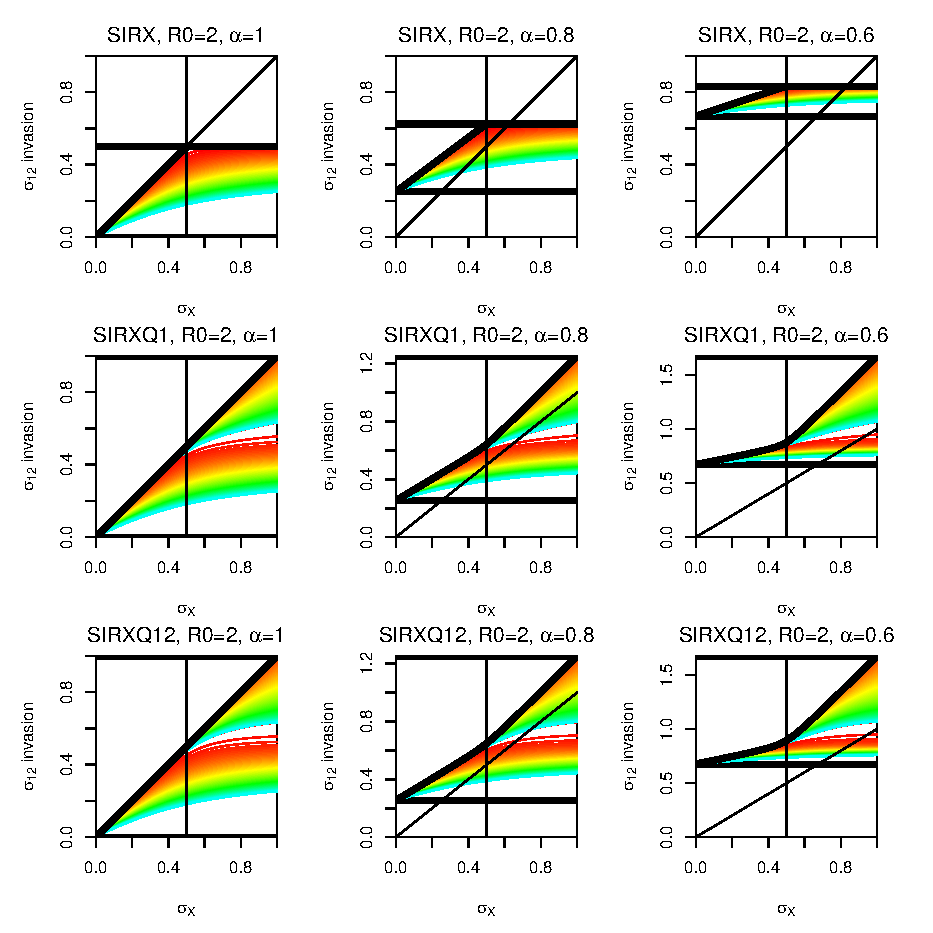
\includegraphics[width=0.8\linewidth]{texte/article3/graph/thresholdn1x_alpha_r02.eps}
  \caption{Invasion threshold. The y-axis represent the minimum
    $\sigma_{12}$ value needed to ensure that the IAU mutant can
    invade a population where a resident IAU is at the endemic
    equilibrium. Columns of figure indicate the effect of functional
    constraint ($\alpha$). Lines of figure present different versions
    of the $SIRX$ model. First line figures: without temporary full
    cross immunity ($Q$) ; second line figures: with $Q$ of duration
    $1/q=6$ months and without immune boosting ($Q1$) ; third line
    figures: with $Q$ ($1/q=6$ months) and immune boosting ($Q12$). In
    each figure, black curves represent the invasion threshold for the
    $SIR$ limit ($g=0$), the $SIRI$ limit ($g \to \infty$) and the
    $SIS$ limit ($g \to \infty$ ; $\sigma_{X}=1$) of the $SIRX$
    model. The $SIRS$ limit correspond to the value
    $\sigma_{X}=1$. Colours represent various values of $g$ from
    $1/g=1$ year (red) to $1/g=70$ years (blue) by 1 year. For second
    and third line figures, additional $1/g$ values are plotted with a
    second colour panel ranging from 0.01 (red) to 1 year (blue) by
    0.01 year.}
  \label{fig:threshold}
\end{figure}


When $\alpha=1$, invasion of the IAU mutant is always possible
whenever $\sigma_{12} > \sigma_{X}$. This sufficient condition (SC) is
not limited to our $SIRX$ model. As we show in the appendix, it
remains true in models allowing for a flexible shape for the evolution
of the reinfection probability within IAU due to gradual antigenic
drift such as the one used by \citet{Xia2005}. From a more biological
standpoint, this SC seems reasonable because it means that infection
by a given IAU confers a better protection against strains belonging
to the same IAU than against strains of another IAU. However, this SC
breaks down as functional constraints ($\alpha<1$) result in an
invasion threshold even when $\sigma_{12} > \sigma_{X}$
(Figure~\ref{fig:threshold}). In the following sections the SC is
always respected.




\section{Transient dynamics of the $SIRX$ model}

%Parameters values:

\subsection{Endemic equilibrium of the 1-IAU $SIRX$ model}

The endemic dynamics of the 1-IAU $SIRX$ model strongly depends on the
value of $g$ and $\sigma_{X}$. We have already shown that in the limit
$\sigma_{X}=1$ the $SIRX$ model is equivalent to the $SIRS$ model
whereas in the limit $g \to \infty$ it reduce to the $SIRI$ model of
\citep{Gomes2004a}. Unlike the $SIRS$ model, the $SIRI$ model presents
a phase transition with a sudden increase in the number of infectious
hosts near $\sigma_{X} = 1/R_0$ (defined as a reinfection threshold).
Figure~\ref{fig:eq_end} shows the evolution of the mean annual attack
rate (estimated on the order of 10\% for seasonal influenza
\citep{Cox2000a}) at the endemic equilibrium in function of $\sigma$
and $g$ for $R_{0}=2$ or 5.

\begin{figure}[!htbp]
  \center
  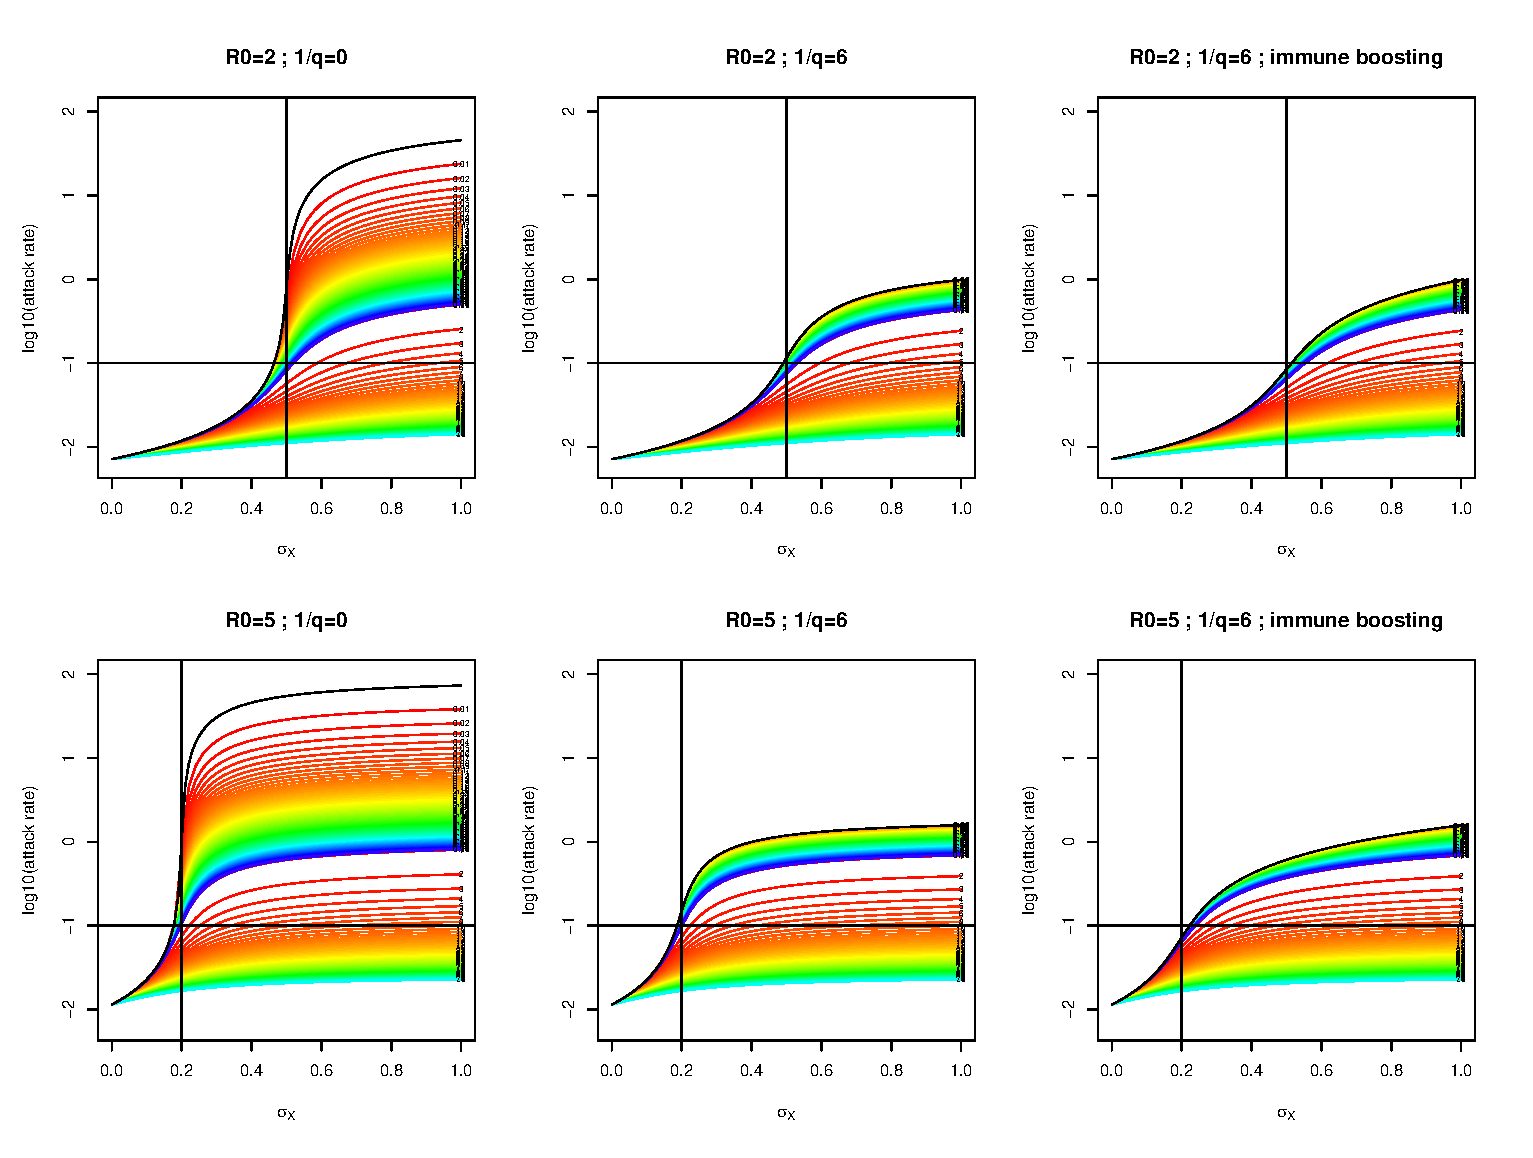
\includegraphics[width=0.7\linewidth]{texte/article3/graph/eq_end.eps}
  \caption{Evolution of the annual attack rate ($\frac{1}{N} \int_0^1
    \nu I(t) dt$) of a single antigenic unit at the endemic
    equilibrium of the $SIRX$ model (first column figures), the
    $SIRXQ1$ model ($1/q=6$ months) (second column figures) and the
    $SIRXQ12$ model ($1/q=6$ months) with immune boosting. Black line
    represent the reinfection limit of the model obtained as $g \to
    \infty$ ; Colours represent various values of $g$. First colour
    panel: $1/g$ varies from 0.01 year (red) to 1 years (blue) by 0.01
    years; second colour panel $1/g$ varies from 1 year (red) to 70
    years (blue) by 1 year.}
  \label{fig:eq_end}
\end{figure}

\subsection{Invasion-replacement dynamics with the 2-IAU $SIRX$ model}
\label{sec:replacement}
We consider the outcome of the invasion of a mutant IAU (indexed by 2)
within a population where a resident IAU (indexed by 1) is at the
endemic equilibrium previously described. Parameter values are the
same for both IAUs and no functional constraints are imposed to the
mutant ($\alpha=1$). Unlike the invasion condition, the outcome of the
invasion depends on the chosen function $f$ for the cross-protection
between IAU. For simplicity we do not assume cumulative effect of the
infection history and we choose the intuitive maximum cross-protection
function $\sigma_{Hk}=\min_{i\in H}\sigma_{ik}$ (see section
\ref{sec:seqeff} for further details). Since the SC is respected it
leads to $\sigma_{Hk}=\sigma_{X}$ when $H=\{1,2\}$ and $k\in\{1,2\}$.
The possible outcomes following invasion are: i) the resident only
goes extinct and it is replaced by the mutant (successful
replacement), ii) the mutant goes extinct and the resident maintains
(failed replacement), iii) both mutant and resident maintain
(coexistence), iv) both mutant and resident go extinct. Since we use
deterministic simulations we fix the extinction threshold at
$10^{-9}$. Figure~\ref{fig:sirx_area} illustrates these different
outcomes for all possible values of $\sigma_{X}$ and $\sigma_{12}$ and
for several values of $R_{0}$ and $g$. Note that for clarity, the
parameter space where the SC is not respected is also represented
($\sigma_{X}>\sigma_{12}$) and then exhibits the invasion threshold
found in section \ref{sec:invasion}.

% As we have already shown, the
%invasion can be prevented when partial protection to the previously
%encountered resident antigenic unit is higher than partial protection
%to a related new antigenic unit ($\sigma > \sigma_x$).  If there is
%not enough evidence to completely discard this case, we think that it
%lacks empirical and intuitive support and will mostly neglect it in
%the following.  We will therefore use the following susceptibility
%reduction the matrix: $\mathbf{M} = \bordermatrix{ & 1 & 2\cr 1 &
%  \sigma & \sigma_x \cr 2 & \sigma_x & \sigma \cr 12 & \sigma & \sigma
%  \cr }$ where $\sigma_x>\sigma$.

\begin{figure}[!htbp]
  \center
  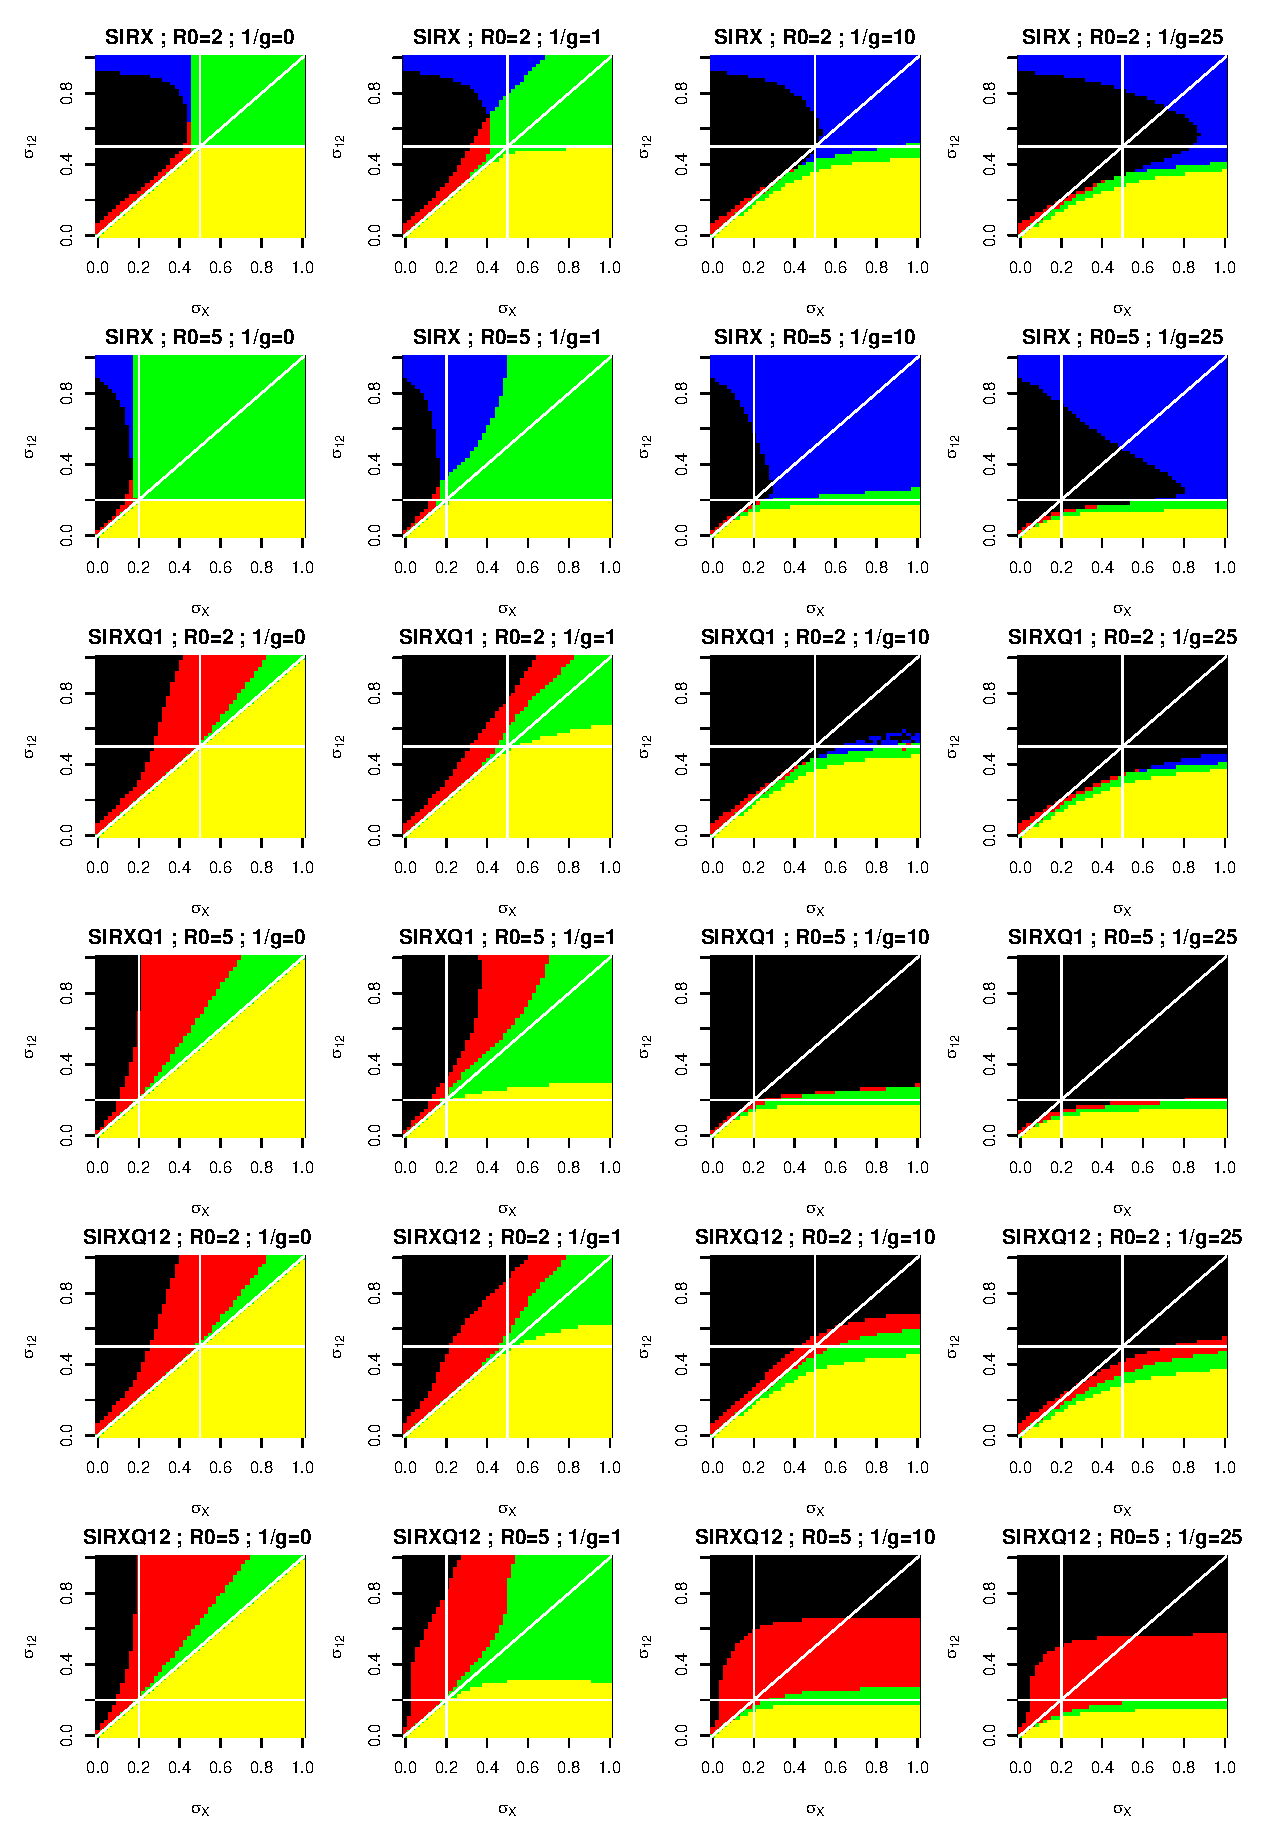
\includegraphics[width=0.8\linewidth]{texte/article3/graph/sens.eps}
  \caption{Outcomes of the transient invasion dynamics described in section \ref{sec:replacement} for the $SIRX$ (first and second line figures), the
    $SIRXQ1$ model ($1/q=6$ months) (third and fourth line figures) and the
    $SIRXQ12$ model ($1/q=6$ months) with immune boosting (fifth and
    sixth line figures). Colours: only the resident goes
    extinct (successful replacement, red), only the mutant goes
    extinct (blue); no IAU goes extinct (coexistence, green), both
    IAU go extinct (black), the
    mutant cannot invade (yellow). White lines indicate the reinfection
    threshold given by $1/R_{0}$.}
  \label{fig:sirx_area}
\end{figure}

Regarding the most interesting replacement area (RA, in red on figure
\ref{fig:sirx_area}) the first striking observation concerns its
smallness compared to other areas. The effects of the different
parameters on its size are the following: i) the RA is maximized when
the tempo of gradual antigenic drift is low ($1/g\thickapprox$ 1 year)
and it is almost nonexistent when $1/g>10$ years. ii) The RA is always
located below the reinfection threshold \textit{i.e.} when
$\sigma_{X}<1/R_{0}$ and consequently the RA decreases when $R_{0}$
increases. As $\sigma_{X} \to \frac{1}{R_0}$ coexistence is observed
instead of replacement. Indeed, since both IAUs benefit a greater
reinfection, the post epidemic extinction risk of the mutant is
reduced but in the same time this latter has less impact on the
resident which maintains (see also the appendix). iii) Finally, regarding the
effect of $\sigma_{12}$, the RA is only observed when the SC is
respected but we also note that the cross-protection within IAU must
not exceed by far the cross-protection between IAUs
($\sigma_{12}\gtrsim\sigma_{X}$). In other words, if we consider
$\Delta\sigma=|\sigma_{12}-\sigma_{X}|$ as a measure of the immune
escape of the mutant IAU over the resident IAU, then this immune
escape cannot exceed a few percents. Moreover, for a fixed value of
$\sigma_{X}<1/R_{0}$, the small RA indicates a high sensitivity to
$\sigma_{12}$ since a too great immune escape leads to the extinction
of both IAUs. This behaviour is confirmed in the appendix where it is
shown that despite the small RA the mutant IAU can produce attack rate
varying from 5 to 50 \%. This range encompasses attack rates observed
during antigenic cluster transition as well as during pandemic
antigenic shifts. Regarding the $SIRS$ limit of our $SIRX$ model (when
$\sigma_{X}=1$) we did not find any RA for any parameter value. On the
opposite, the $SIRI$ limit (when $g\to\infty$) exhibits the same RA
characteristics than the $SIRX$ model when $g>1\text{ }year^{-1}$.
These characteristics were previously reported by
\citet{Goekaydin2007} and this preliminary study on the $SIRX$ model
emphasizes the importance of the reinfection threshold for the
replacement of IAU.

In the following section we fix $R_0=2$ (as most of $R_0$ estimates
are within the range 1.5-2 \citep{Lessler2007}) and $1/g=1$ year
(found to generally maximise the RA) and we consider $\sigma_{X}$
values sufficiently high to ensure attack rates of the order of 10\%.
As revealed by figure~\ref{fig:eq_end} this last condition imposes to
take $\sigma_{X}$ smaller but close to the reinfection threshold. In
accord with \citet{Goekaydin2007}, we find that other values of $R_0$
in the range 1.5-5 do not alter the results provided that $\sigma_{X}$
is adapted to be smaller but close to $1/R_0$.


\subsection{Metapopulation dynamics and seasonality}

In order to study IAU replacement in a more realistic setting, we
incorporate the $SIRX$ model of eq~\eqref{eq:full} into a stochastic
metapopulation framework as depicted in
equation~\eqref{eq:full_metapop} where $\{c_l\}_{l\in\{1..L\}}$
denotes the set of the $L$ cities.

\begin{footnotesize}
  \begin{align}
    \label{eq:full_metapop}
    \dot{R_{c_l}}_{\begin{subarray}{l}\varnothing \\ \varnothing \end{subarray}} &= \mu_{c_l} N_{c_l} -\sum_k \beta_k(t) {R_{c_l}}_{\begin{subarray}{l}\varnothing \\ \varnothing \end{subarray}} \frac{I_{c_l}^k}{N_{c_l}} - \mu_{c_l} {R_{c_l}}_{\begin{subarray}{l}\varnothing \\ \varnothing \end{subarray}}\\
%%
    \dot{R_{c_l}}_{\begin{subarray}{l}H\\ J \end{subarray}} &= \sum_{k
      \in J} \beta_k \sigma_{Hk} {R_{c_l}}_{\begin{subarray}{l}H \\ J
        \setminus k \end{subarray}} \frac{I_{c_l}^k}{N_{c_l}} -\sum_{k
      \notin J} \beta_k(t) \sigma_{Hk}
    {R_{c_l}}_{\begin{subarray}{l}H\\ J \end{subarray}}
    \frac{I_{c_l}^k}{N_{c_l}} - \sum_{k \in J} g_k
    {R_{c_l}}_{\begin{subarray}{l}H\\ J \end{subarray}} + \sum_{k \in
      \{H \setminus J\}} g_k {R_{c_l}}_{\begin{subarray}{l}H\\ J\cup
        k \end{subarray}} -\mu_{c_l}
    {R_{c_l}}_{\begin{subarray}{l}H\\J \end{subarray}} \notag \\
%%
    \dot{I_{c_l}}^k &= \sum_{\begin{subarray}{l}H \subseteq \mathbf{K}
        \\ J \subseteq \{H \setminus k \} \end{subarray}}
    {R_{c_l}}_{\begin{subarray}{l}H \\ J \end{subarray}}
    \frac{I_{c_l}^k}{N_{c_l}} -\nu I_{c_l}^k -\mu_{c_l} I_{c_l}^k
    -\sum_{m\neq l} \frac{\tau_{c_lc_m}}{N_{c_l}} I_{c_l}^k
    +\sum_{m\neq l} \frac{\tau_{c_mc_l}}{N_{c_l}} I_{c_m}^k \notag
  \end{align}
\end{footnotesize}

For simplicity, only infectious hosts are allowed to travel,
$\frac{\tau_{c_mc_l}}{N_{c_l}}$ being the probability that a host
located in city $c_l$ of size $N_{c_l}$ travels to city $c_m$.
Eq~\eqref{eq:full_metapop} was simulated on a network of 52 global
cities (depicted in the appendix) linked by air transportation data
from year 2000 and published in \citep{Grais2003}. Population sizes of
each city were taken from http://unstats.un.org/unsd/demographic/.
Seasonal forcing was introduced for cities in temperate areas with a
sinusoidal varying transmission rate $\beta(t)= \frac{1}{2} \left[
  (1-\frac{\beta_{min}}{\beta_{max}}) \sin(2 \pi
  \frac{(t-t_{max})}{365}+\frac{\pi}{2}) +1
  +\frac{\beta_{min}}{\beta_{max}} \right]$ with phase opposition for
North and South hemisphere (\citep{Finkelman2007}). No seasonal
forcing was assumed in the tropics as transmission appears to be more
constant \citep{Viboud2006}.

\subsubsection{Invasion-replacement in the stochastic metapopulation model}

We applied a similar invasion protocol as in the deterministic
framework of section \ref{sec:replacement}.
Figure~\ref{fig:sirx_s03_039} (see also the appendix.) reveals that
simulations of the stochastic metapopulation model are in good
agreement with the previously studied deterministic model. Indeed, the
RA is maximised when $\sigma_{X}$ is close to $1/R_0$. Moreover, as
$\sigma_{X}$ approaches $1/R_0$, coexistence substitutes replacement
and higher values of $\sigma_{12}$ are needed to ensure the resident
IAU replacement by the mutant one.

The appendix reveal that we also find a high sensitivity to the immune
escape $\Delta\sigma$ of the mutant. $\Delta\sigma\approx2\%-3\%$ are
sufficient to ensure successful antigenic unit replacement whereas
higher values result in unrealistic high epidemics (within a few
percent of immune escape the ratio of the maximum epidemic size of the
mutant over the resident was found to vary from 1 to 100) .

\begin{figure}[htp]
  \center
  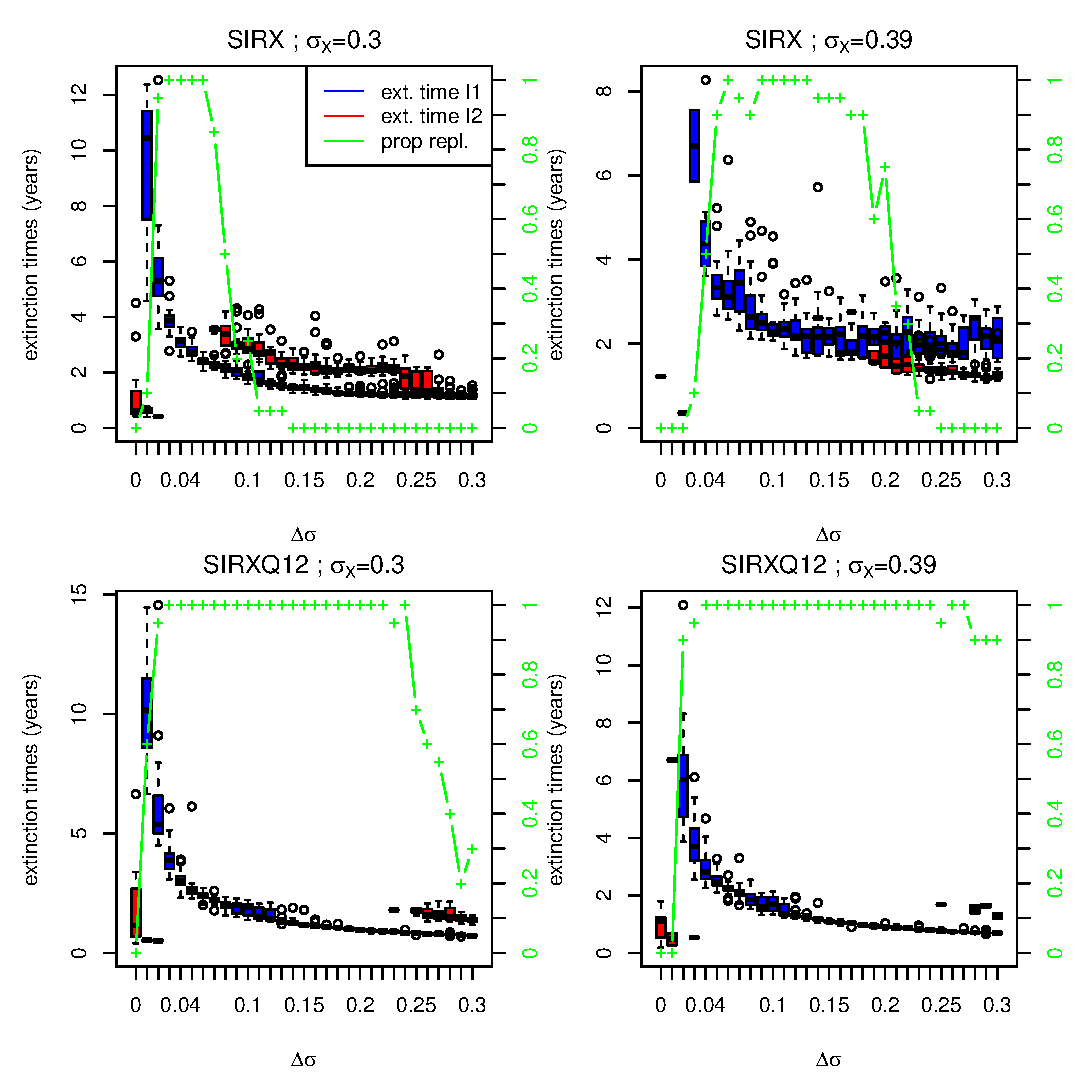
\includegraphics[width=0.7\linewidth]{texte/article3/graph/sirx_s03_039_final.eps}
  \caption{Replacement area (RA) for 20 realisations of the stochastic
    $SIRX$ model (first line figures) and $SIRXQ12$ with immune boosting (second line)
    metapopulation model . The mutant antigenic unit (red) is
    introduced in april 1$^{st}$ in Shenzen.  Parameters: $R_0=2$; $1/\nu=4$ days ; $1/g=1$
    year; $\sigma_{X}=0.3$
    (top) or $\sigma_{X}=0.39$ (bottom, chosen to maximize the RA). No seasonal forcing is assumed in the tropics and northern
    and southern hemisphere are forced with phase opposition
    ($t^{north}_{max}= 356$, $t^{south}_{max}= 173$) with intensity
    $\frac{\beta_{min}}{\beta_{max}}=0.4$.}
  \label{fig:sirx_s03_039}
\end{figure}


\subsubsection{Sequential effect}
\label{sec:seqeff}
We extend the previous analysis by considering the successive emergence of
IAUs. When three or more IAUs are co-circulating it is
necessary to specify the general function $f$ that defines the cross-protection conferred by previous IAU exposures against infection by new IAUs. As stated by \citet{Adams2007a}, very
little empirical information relating to the shape of $f$ is available and most
previous models have used either a minimum or a multiplicative function.  The
minimum function assumes that only antibodies to the most related IAU of the host immune repertoire are produced. The multiplicative function assumes
that antibodies of the entire host immune repertoire are produced and their net
benefit is greater than either one of them alone. In reality, host immune response should lie between these two extrema. However, as the minimum
function is the most extensively used by previous models and in the absence
of any strong evidence for an alternative function, we choose to use it in
this study.

The cross-protection factor $\sigma_{Hk}$ is thus the same as the one previously described in section \ref{sec:replacement}: $\sigma_{Hk}=\min_{i\in H}\sigma_{ik}$ and since all IAUs have the same reinfection parameter $\sigma_{Hk}=\sigma_{X}$ if $k\in H$.

The specific cross-protection factor $\sigma_{ik}$ encapsulates the
evolution of antigenic distance between two IAUs where $i$ and $k$
refer to the order of emergence of both IAUs. Various forms can be
chosen to describe this evolution but they are not without strong
consequences \citep{Adams2007a}. As a simple starting point, we will
consider a linear function by assuming that $\sigma_{ik} = \sigma_{X}
+ \Delta\sigma |k-i|$ where $|k-i|$ is the kinship level between IAU
$i$ and IAU $k$. In agreement with experimental studies on influenza
A/H3N2 antigenic clusters (\citet{Smith2004}), IAUs are sequentially
introduced every 4 years in Shenzen on april $1^{st}$ with an initial
seed of 100 infected hosts to prevent stochastic extinctions at the
beginning of the invasion.

Simulations of the 5-IAUs $SIRX$ stochastic metapopulation model
confirm the high sensitivity of the model to $\Delta\sigma$. Immune
escapes greater than 5\% lead to unrealistic high epidemics as well as
too long refractory periods compared to data
(figure~\ref{fig:world_sirx} illustrates the effect of an increasing
sequence of $\Delta\sigma$). As shown in the appendix, simulations
where $\sigma_{X} \to \frac{1}{R_0}$ exhibit long periods of
coexistence with old IAUs being maintained at low incidence.

\begin{figure}[!htbp]
  \center
  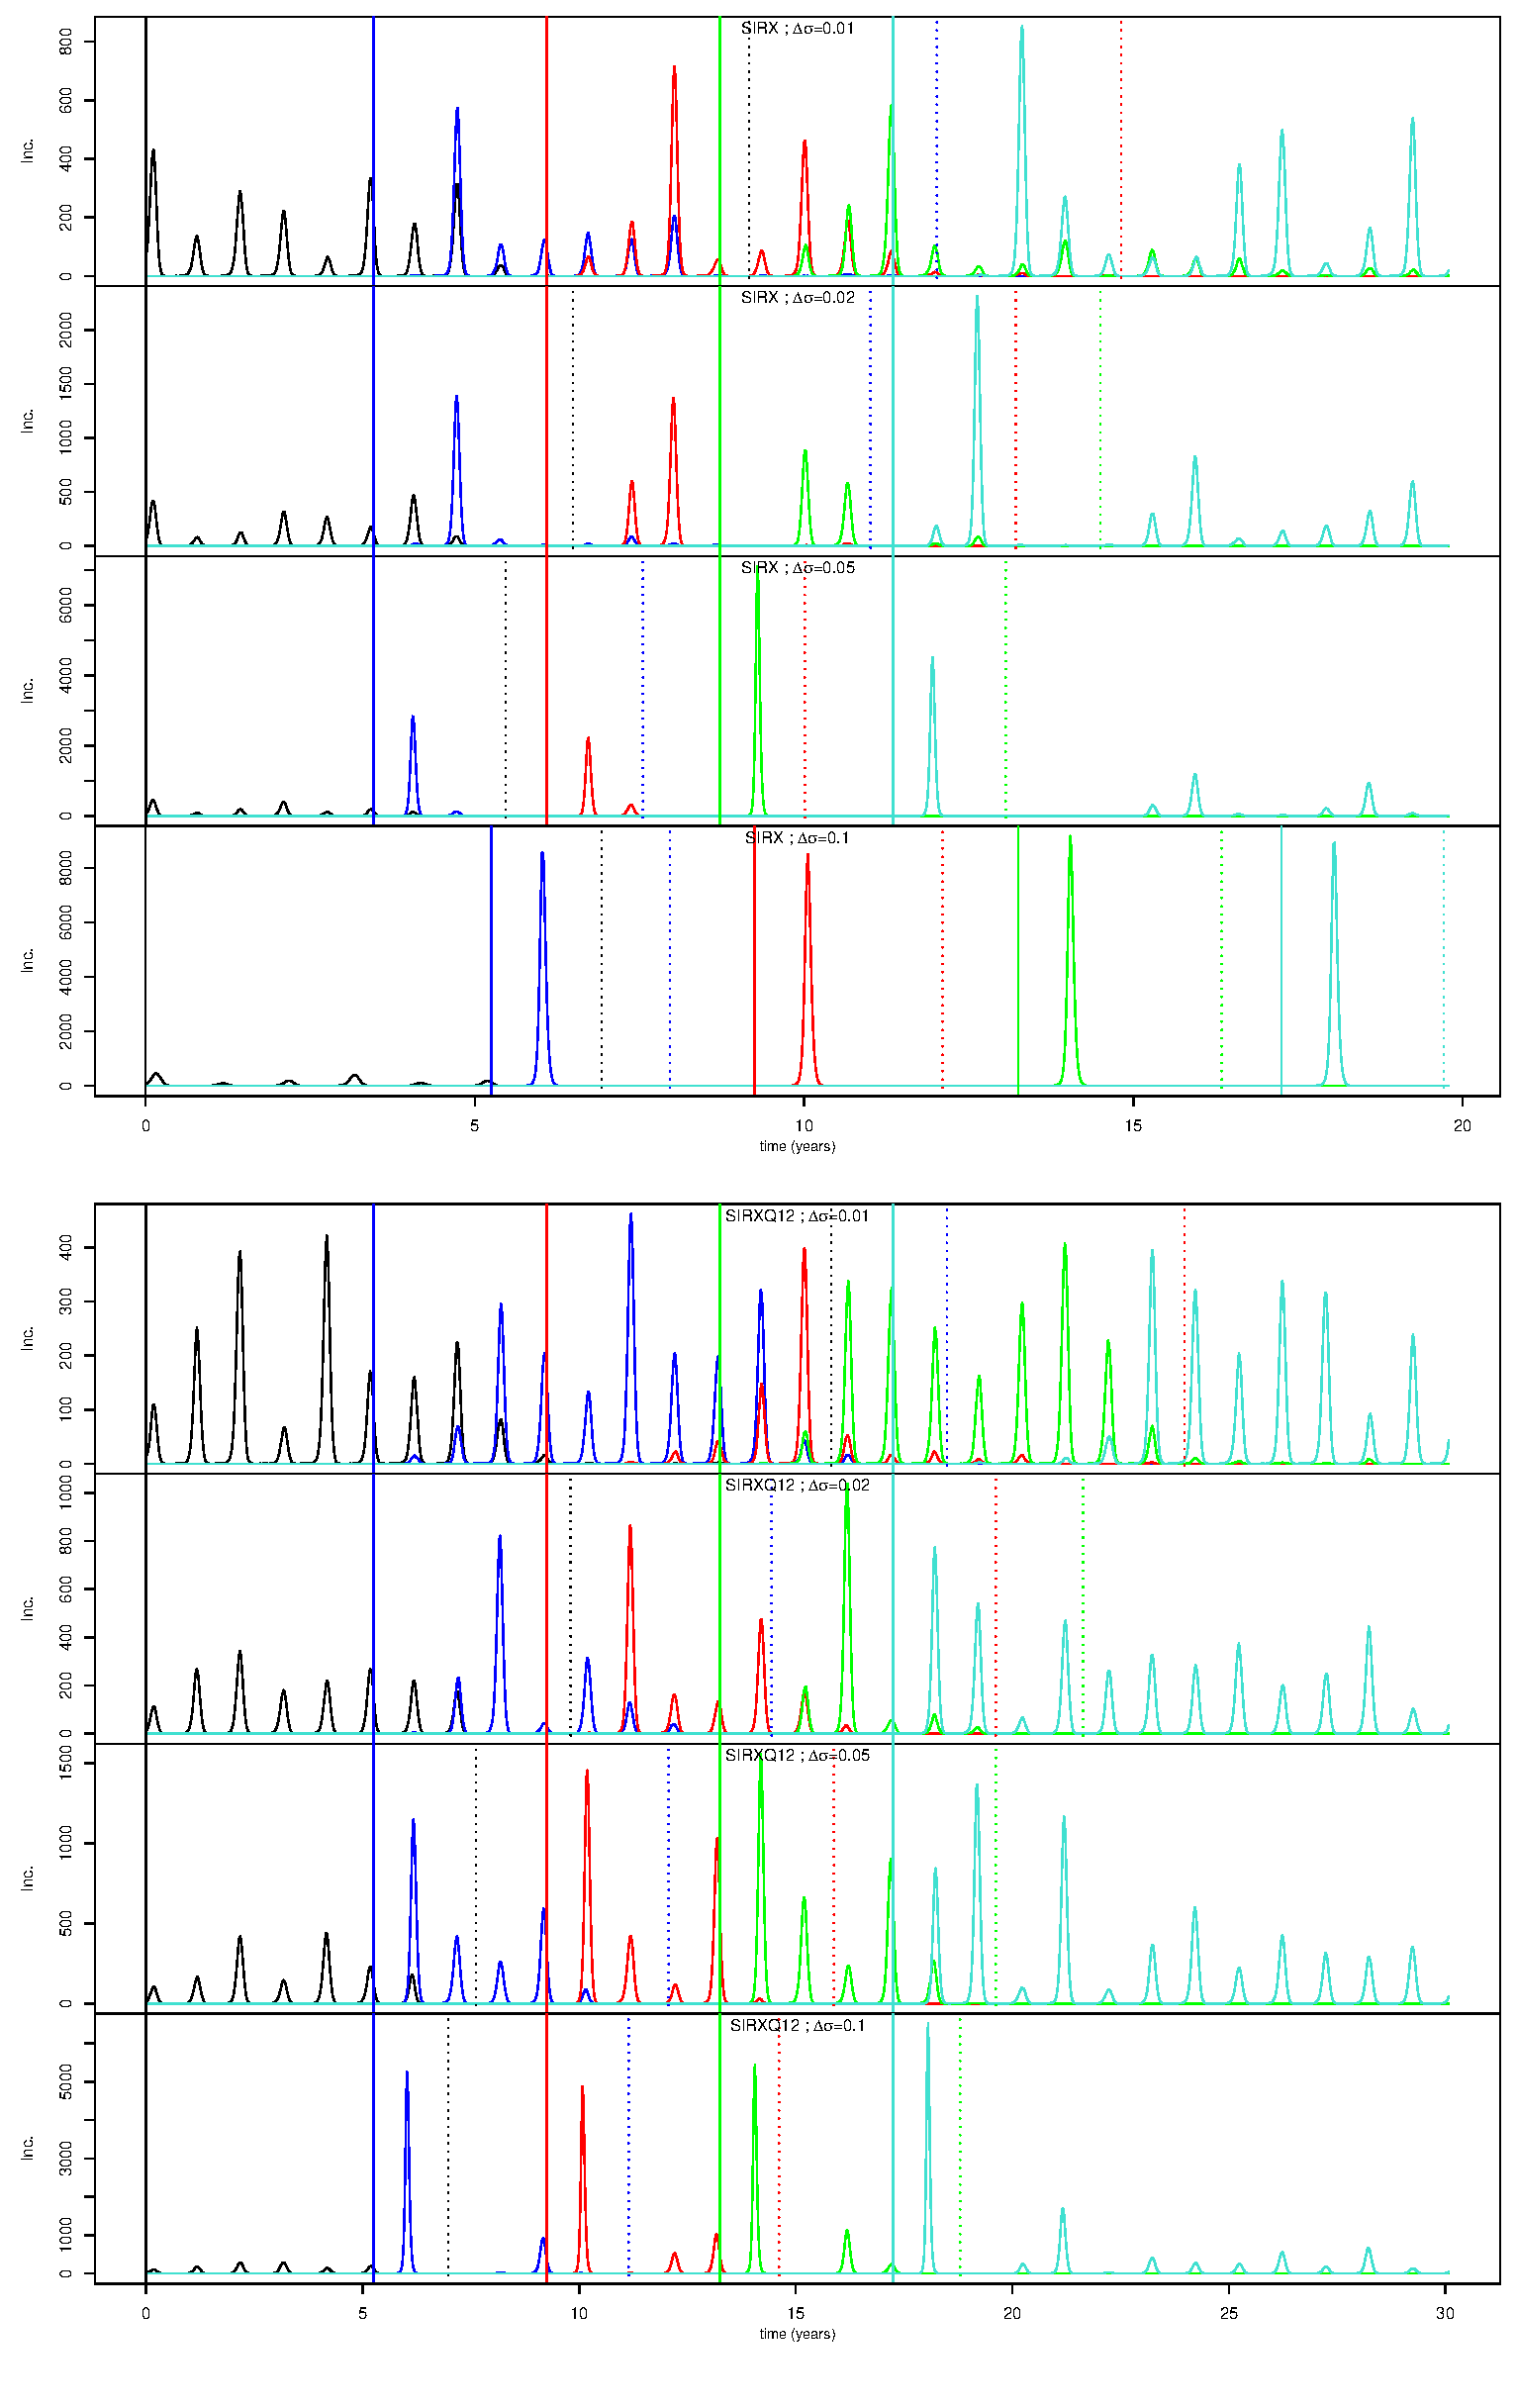
\includegraphics[width=0.8\linewidth]{texte/article3/graph/traj_metapop.eps}
  \caption{Typical realisation of the $SIRX$ model (top panel) and
    $SIRXQ12$ model (bottom panel) with immune boosting in the
    stochastic metapopulation framework in the city of Paris. First
    IAU is at the endemic equilibrium and 4 other IAUs are
    sequentially introduced every 4 years in Shenzen on april 1$^{st}$
    with an initial seed of 100 infected hosts. y-axis is weekly
    incidence per 100 000 inhabitants. Parameters: $\sigma_{X}=0.3$
    and $\Delta\sigma\in\{0.01, 0.02, 0.05, 0.1\}$. Other parameters
    are identical to figure~\ref{fig:sirx_s03_039}. Vertical plain
    (dotted) lines correspond to the introduction (worldwide
    extinction) times of the IAUs coded by colours. Corresponding
    annual attack rates are plotted in the appendix.}
  \label{fig:world_sirx}
\end{figure}

In summary, realistic antigenic cluster replacement with the $SIRX$
model appears possible only for a small range of cross-immunity
parameters ($\sigma_{X}$ and $\Delta\sigma$). We have seen that to
ensure recurrent epidemics with attack rates comparable to data, the
reinfection parameter of each IAU ($\sigma_{X}$) must be smaller but
close to $1/R_0$. Furthermore, for a fixed value of $\sigma_{X}$, the
epidemic size of a newly introduced IAU is highly sensitive to its
immune escape since $\Delta\sigma>5\%$ results in unrealistic high
epidemic size followed by too long refractory periods. On the other
hand, when $\Delta\sigma< 5 \%$ our $SIRX$ model is able to reproduce
the patterns observed in real data. Recently, \citet{Finkenstaedt2005}
have obtained similar estimates of immune escape intensity in a study
using french influenza-like illness data as well as a model allowing
for both gradual and punctuated renewal of susceptible. Despite
conceptual differences between our two models, their punctuated immune
escape estimates can be related to our $\Delta\sigma$ parameter. Their
results show that punctuated immune escape are all smaller than 7\%
with 53\% of the estimates $\leq 2\%$, 26.7\% between 2 and 5 \% and
20\% between 5 and 7 \%, which is in accordance with the values needed
by the $SIRX$ model. However, \citet{Finkenstaedt2005} found 15
discrete antigenic jumps between the years 1985 and 2002, a pattern
more related to noisy gradual antigenic drift than to rarer antigenic
cluster transitions (on average, clusters remained dominant for 3.3
years \citep{Smith2004}).

From our side, the small amount of immune escape between IAUs when
compared with the high amount of reinfection within IAU ($\Delta\sigma
<< \sigma_{X}$) seems not in agreement with previous studies on
cross-protection and influenza A/H3N2 antigenic clusters. In 2004,
\citeauthor{Smith2004} have presented a 2D antigenic map of 273 viral
isolates of human influenza A/H3N2. Their study reveals that strains
tend to group in clusters rather than to form a continuous antigenic
lineage. Since cross-immunity is closely related to antigenic
distance, it is expected that cross-immunity within clusters is much
higher than cross-immunity between clusters. For instance
\citet{Koelle2009} considered a 60-80 \% degree of cross-immunity
between successive antigenic clusters and a full cross-immunity
between strains belonging to the same cluster. With our notations, it
amounts to considering $\sigma_{X}=0$ and
$\sigma_{ij}=\sigma_{X}+\Delta\sigma|i-j|=\Delta\sigma=20-40\%$ where
$i$ and $j$ are two successive IAUs. Figure \ref{fig:sirx_area}
reveals that within this parameter range IAU replacement is impossible
and complete extinction of both IAUs is observed (see also the
appendix). 

A more detailed discussion on the scale of $\Delta$ can be found in
the discussion. In the next sections, we introduce factors that
increase the range of immune escape leading to successful IAU
replacement.


\subsection{Functional constraints and evolutionary trade-off between
  immune escape and transmission}

There is large evidence for functional constraints and evolutionary
trade-off associated with IAU transitions \citep{Rambaut2008}.
Figure~\ref{fig:threshold} reveals that $\alpha<1$ impairs invasion of
a mutant IAU even if $\sigma_{12}>\sigma_{X}$. Functional constraints
can then result in higher values for $\Delta\sigma$ but it
nevertheless remains to test to what extent a resident IAU can be
replaced by an intrinsically less fit IAU mutant. The situation is all
the more complicated to model as compensatory mutations are expected
in nature. We address the question in a simple way by only examining
the mutant invasion, assuming that the $\alpha$ parameter remains
constant during the initial outbreak.

\begin{figure}[!htbp]
  \center
  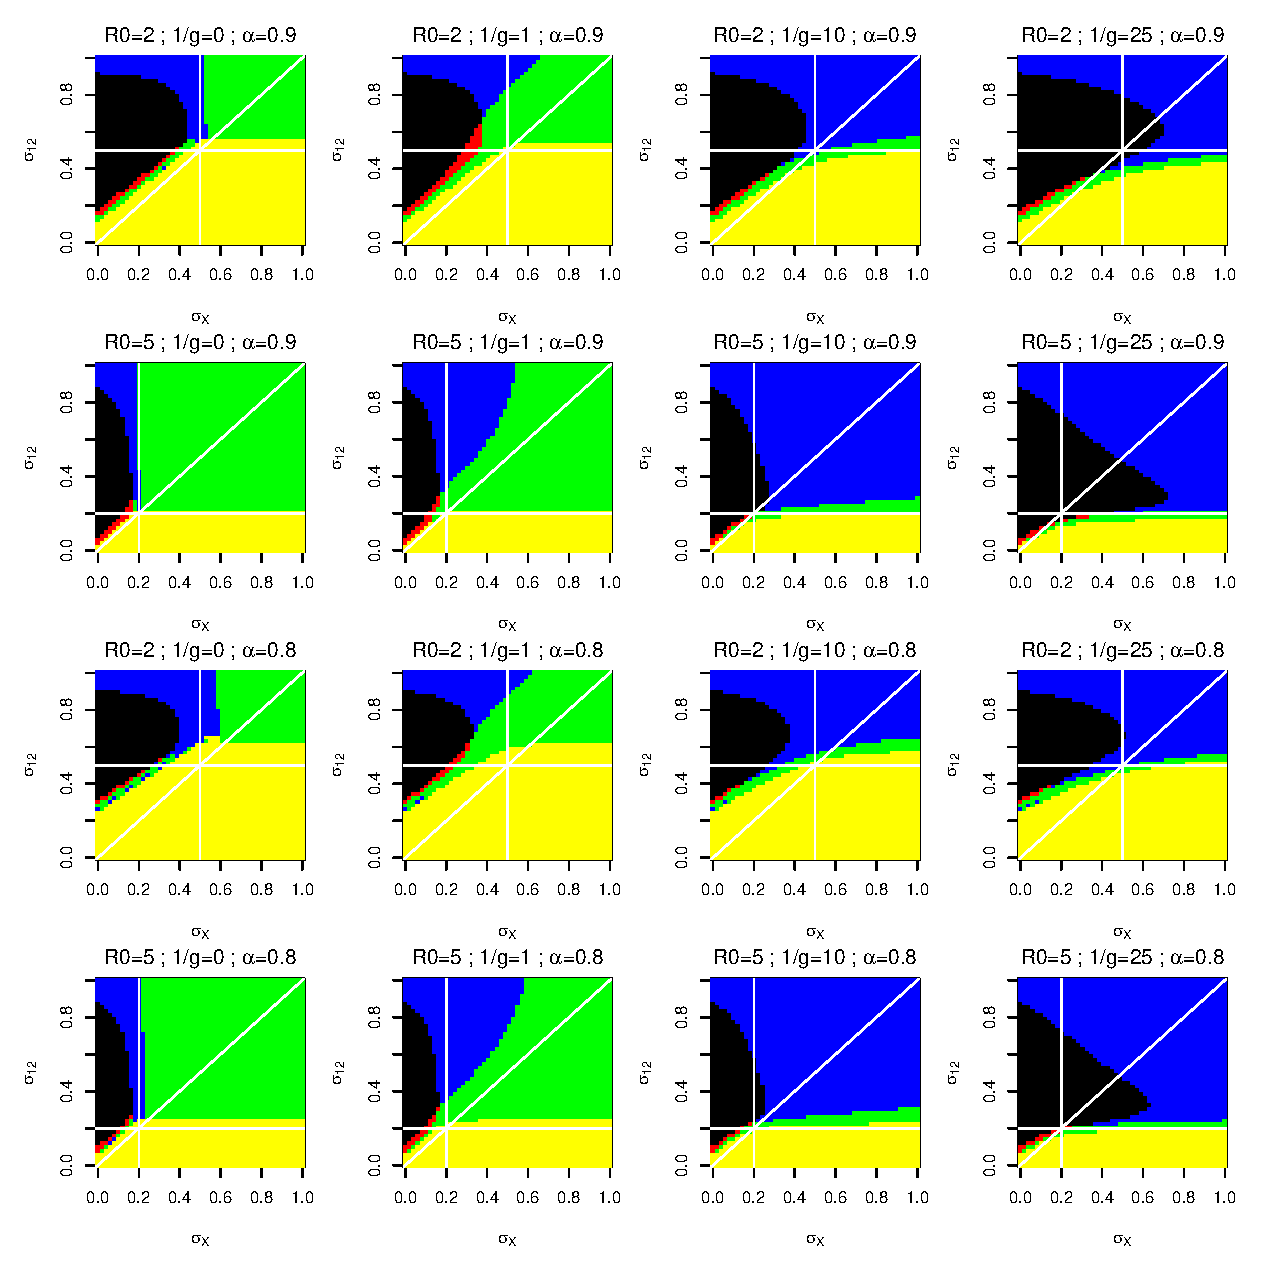
\includegraphics[width=0.8\linewidth]{texte/article3/graph/sirx_trade_off_short.eps}
  \caption{Effect of functional constraints ($\alpha\in\{0.9,0.8\}$)
    on the invasion outcome of a mutant IAU within a population where
    a resident IAU is at the endemic equilibrium for the $SIRX$ model.
    Color legend is identical as figure~\ref{fig:sirx_area}}
  \label{fig:sirx_trade_off_09}
\end{figure}

Figure~\ref{fig:sirx_trade_off_09} (see also the appendix) reveal that
the functional constraints translate the RA into greater
$\Delta\sigma$ values and allow higher antigenic distance between
successive IAUs. In the other hand, the RA is significantly narrow
comparing to figure \ref{fig:sirx_area} and new coexistence areas are
observed. Given the existing variability observed in immune escape
intensity such a situation can result in alternate periods of
coexistence and replacement. However, the full study of this pattern
will require a way to model compensatory mutations which is beyond the
scope of this paper.


\section{Temporary period of IAU-transcending immunity}


\subsection{Biological hypothesis}
\label{sec:Q}

The existence of a period of temporary full protection against infection by any strain was
originally proposed by \citet{Webster1992} to explain subtype
replacement during pandemics \textit{i.e.} when partial
cross-protection ensured by anti-HA and NA antibodies is low.
\citet{Webster1992} suggested that such full protection
could be mediated by CD8+ T-lymphocyte response to the shared internal
proteins among human influenza A virus.

\citet{Webster1992} prediction was confirmed by \citet{Ferguson2003}
who also revealed that this period was of tremendous importance to
restrict strain diversity during seasonal influenza in absence of
antigenic clusters. These results were analysed by \citet{Tria2005}
who argued that temporary strain-transcending immunity could only
restrict strain diversity if it was coupled with a source of
heterogeneity. One important difference between \citet{Ferguson2003}
and \citet{Tria2005} individual based model was the way this period
was introduced. In \citet{Ferguson2003} study, following exposure to a
strain $s$ (due to a close contact with an infectious host) the
probability of becoming infected depends on the strain $s$ and the
host's immune repertoire $H$. But whatever the outcome of the
exposure, the host acquires a short-lived strain-transcending immunity
that we can mechanistically represent by a new class $Q$ of expected
duration $1/q=6$ months. However, for a better understanding of what
is ``doing'' the $Q$ class we must detail the three ways a host enters
it following exposure:
\begin{enumerate}
\item if $s\notin H$ and $H$ fails to confer sufficient
  cross-protection, the host becomes infected, updates $H\rightarrow
  H\cup\{s\}$ and enters the $Q$ class (case $Q_{1}$)
\item if $s\notin H$ and $H$ confers sufficient cross-protection, the
  host escapes infection he does not updates $H$ and enters the $Q$
  class (case $Q_{2}$)
\item if $s\in H$ the host escapes infection and enters the $Q$ class
  (case $Q_{3}$)
\end{enumerate}

The biological justification of $Q_{1}$ implies triggering of cellular
immunity following infection, a process confirmed in various animals
models \citep{Grebe2008} whereas $Q_{2}$ and $Q_{3}$ refer to the
immune boosting assumption \citep{Ferguson2003}. This interpretation
is discussed further in the discussion. By contrast,
\citet{Tria2005} implemented only the case $Q_{1}$. As we show in
the following, this could be responsible for the differing conclusions
between the two models.

Figure \ref{Q123} illustrates the three assumptions on the $Q$ class
in the context of IAU instead of strains as used in this paper.

\begin{figure}[htbp]
\begin{center}
\begin{tikzpicture}[node distance=3cm, auto,>=latex', thick]
  \tikzstyle{sebQ3}=[rectangle, fill=red, draw=gray, text=black]
  \tikzstyle{sebQ}=[rectangle, fill=red!20, draw=gray, text=black]
  \tikzstyle{seb}=[rectangle, fill=blue!20, draw=gray, text=black]
  \node [seb] (X_1_1) {$R_{\begin{subarray}{l}H \\ J\end{subarray}}$};
  \node [seb, right of=X_1_1,node distance=3cm] (I_2_1_1) {$I^{k}_{\begin{subarray}{l}H \\J\end{subarray}}$};
  \node [sebQ, right of=I_2_1_1,node distance=2cm] (Q_12_12) {${Q_1}_{\begin{subarray}{l}H(\cup k) \\J\cup k\end{subarray}}$};
  \node [sebQ, below of=X_1_1,node distance=2cm] (Q2_1_1) {${Q_2}_{\begin{subarray}{l}H \\J\end{subarray}}$};
  \node [sebQ3, above of=X_1_1,node distance=2cm] (Q3_1_1) {${Q_3}_{\begin{subarray}{l}H \\J\end{subarray}}$};
  \node [seb, right of=Q_12_12,node distance=2cm] (X_12_12) {$R_{\begin{subarray}{l}H(\cup k) \\J\cup k\end{subarray}}$};
  
  \draw [->] (X_1_1) --node {$\beta \sigma^k_{H} I^{k:k \notin J}$} (I_2_1_1);
  \draw [->] (X_1_1) edge[bend right]node[left] {$\beta (1-\sigma^k_{H})I^{k:k \notin J}$} (Q2_1_1);
  \draw [->] (Q2_1_1) edge[bend right]node[right] {$q$} (X_1_1);
  
  \draw [->] (X_1_1) edge[bend left]node[left] {$\beta  I^{k:k \in J}$} (Q3_1_1);
  \draw [->] (Q3_1_1) edge[bend left]node[right] {$q$} (X_1_1);
  
  \draw [->] (I_2_1_1) --node{$\nu$}(Q_12_12);
  \draw [->] (Q_12_12) --node{$q$}(X_12_12);
\end{tikzpicture}
\caption{Three mechanisms for the temporary period of IAU-transcending
  immunity (red boxes). When exposed to an IAU $k$ that does not
  belong to the effective immune repertory $J$ ($k \notin J$) , hosts
  enter $Q_{1}$ after infection whereas they enter $Q_{2}$ if their
  immune history $H$ succeed in conferring immunity against $k$ (and
  therefore avoid the infection). Hosts protected to $k$ due to
  effective immunity ($k \in J$) always escape infection but
  nevertheless enter $Q_{3}$ after an exposure.}
\label{Q123}
\end{center}
\end{figure}

\clearpage




\subsection{Extension of the simple $SIRX$ model}

Eq. \eqref{eq:fullQ} extends eq. \ref{eq:full} to incorporate the
assumption of temporary IAU-transcending immunity under case $Q_{1}$.
Note also that co-infection is not allowed anymore. This model is
labeled $SIRXQ_{1}$.

\begin{footnotesize}
  \begin{align}
    \label{eq:fullQ}
    \dot{R}_{\begin{subarray}{l}\varnothing \\
        \varnothing \end{subarray}} &= \mu N -\sum_k \beta_k(t) R_{\begin{subarray}{l}\varnothing \\ \varnothing \end{subarray}} \frac{I^k}{N} - \mu R_{\begin{subarray}{l}\varnothing \\ \varnothing \end{subarray}}\\
  %% 
    \dot{I}^k_{\begin{subarray}{l}H\\ J \setminus k \end{subarray}} &=
    \beta_k(t) \sigma_{Hk} R_{\begin{subarray}{l}H \\ J\setminus
        k \end{subarray}} \frac{I^k}{N} -\nu I^k_{\begin{subarray}{l}H
        \\ J \setminus k \end{subarray}} -\sum_{m \in J \setminus k}
    g_m I^k_{\begin{subarray}{l}H \\ J \setminus k \end{subarray}} +
    \sum_{m \in (H \setminus (J \cup k))} g_m
    I^k_{\begin{subarray}{l}H \\ (J \setminus k) \cup
        m \end{subarray}}
    -\mu I^k_{\begin{subarray}{l}H \\ J \setminus k \end{subarray}} \notag \\
  %% 
    \dot{Q}_{\begin{subarray}{l}H\\ J \end{subarray}} &= \sum_{k \in
      J} \nu I^k_{\begin{subarray}{l}H \setminus k \\ J \setminus
        k \end{subarray}} +\sum_{k \in J} \nu
    I^k_{\begin{subarray}{l}H \\ J \setminus k \end{subarray}} -q
    Q_{\begin{subarray}{l}H \\ J\end{subarray}} -\sum_{m \in J} g_m
    Q_{\begin{subarray}{l}H \\ J\end{subarray}} + \sum_{m \in (H
      \setminus J )} g_m Q_{\begin{subarray}{l}H \\ J \cup
        m \end{subarray}} -\mu
    Q_{\begin{subarray}{l}H \\ J \end{subarray}} \notag \\
  %% 
    \dot{R}_{\begin{subarray}{l}H\\ J \end{subarray}} &= q
    Q_{\begin{subarray}{l}H \\ J\end{subarray}} -\sum_{k \notin J}
    \beta_k(t) \sigma_{Hk} R_{\begin{subarray}{l}H\\ J \end{subarray}}
    \frac{I^k}{N} - \sum_{m \in J} g_m R_{\begin{subarray}{l}H\\
        J \end{subarray}} + \sum_{m \in (H \setminus J)} g_m
    R_{\begin{subarray}{l}H\\ J\cup m \end{subarray}} -\mu
    R_{\begin{subarray}{l}H\\J \end{subarray}} \notag
  \end{align}
\end{footnotesize}


where $$I^k=\sum_{\begin{subarray}{l}H \subseteq \mathbf{K} \\ J
    \subseteq H \end{subarray}} I^k_{\begin{subarray}{l}H\\ J
    \setminus k \end{subarray}}$$.

and the number of equations is given by: $$2 \sum_{k=0}^{N_K} \left
  (\binom{N_K}{k} \sum_{p=0}^k \binom {k}{p} \right) + \sum_{k=0}^{N_K}
\left( \binom{N_K}{k} \sum_{p=0}^k \binom{k}{p}(N_K-p) \right ) $$

In order to investigate the additional effect of assumption $Q_{2}$ we
modify eq \eqref{eq:fullQ} and obtain eq \eqref{eq:fullQferg}. The
corresponding model is labeled $SIRXQ_{12}$.

\begin{footnotesize}
  \begin{align}
    \label{eq:fullQferg}
    \dot{R}_{\begin{subarray}{l}\varnothing \\
        \varnothing \end{subarray}} &= \mu N -\sum_k \beta_k(t) R_{\begin{subarray}{l}\varnothing \\ \varnothing \end{subarray}} \frac{I^k}{N} - \mu R_{\begin{subarray}{l}\varnothing \\ \varnothing \end{subarray}}\\
%%
    \dot{I}^k_{\begin{subarray}{l}H\\ J \setminus k \end{subarray}} &=
    \beta_k(t) \sigma_{Hk} R_{\begin{subarray}{l}H \\ J\setminus
        k \end{subarray}} \frac{I^k}{N} -\nu I^k_{\begin{subarray}{l}H
        \\ J \setminus k \end{subarray}} -\sum_{m \in J \setminus k}
    g_m I^k_{\begin{subarray}{l}H \\ J \setminus k \end{subarray}} +
    \sum_{m \in (H \setminus (J \cup k))} g_m
    I^k_{\begin{subarray}{l}H \\ (J \setminus k) \cup
        m \end{subarray}}
    -\mu I^k_{\begin{subarray}{l}H \\ J \setminus k \end{subarray}} \notag \\
%%
    \dot{Q}_{\begin{subarray}{l}H\\ J \end{subarray}} &= \sum_{k \in
      J} \nu I^k_{\begin{subarray}{l}H \setminus k \\ J \setminus
        k \end{subarray}} +\sum_{k \in J} \nu I^k_{\begin{subarray}{l}H \\
        J \setminus k \end{subarray}} -q Q_{\begin{subarray}{l}H \\ J
      \end{subarray}} -\sum_{m \in J } g_m Q_{\begin{subarray}{l}H \\
        J \end{subarray}} + \sum_{m \in (H \setminus J)} g_m
    Q_{\begin{subarray}{l}H \\ J \cup m \end{subarray}} -\mu
    Q_{\begin{subarray}{l}H \\ J \end{subarray}} \notag \\
%%
    \dot{Q'}_{\begin{subarray}{l}H\\ J \end{subarray}} &= \sum_{k
      \notin J} -\beta_k(t) (1 -\sigma_{Hk}) R_{\begin{subarray}{l}H\\
        J \end{subarray}} \frac{I^k}{N} -q Q'_{\begin{subarray}{l}H \\
        J \end{subarray}} -\sum_{m \in J} g_m Q'_{\begin{subarray}{l}H
        \\ J \end{subarray}} + \sum_{m \in (H \setminus J)} g_m
    Q'_{\begin{subarray}{l}H \\ J \cup m \end{subarray}} -\mu
    Q'_{\begin{subarray}{l}H \\ J \end{subarray}} \notag \\
%%
    \dot{R}_{\begin{subarray}{l}H\\ J \end{subarray}} &= q
    Q_{\begin{subarray}{l}H \\ J \end{subarray}} +q
    Q'_{\begin{subarray}{l}H \\ J \end{subarray}} +\sum_{k \notin J}
    -\beta_k(t) R_{\begin{subarray}{l}H\\ J \end{subarray}}
    \frac{I^k}{N} - \sum_{m \in J} g_m R_{\begin{subarray}{l}H\\
        J \end{subarray}} + \sum_{m \in (H \setminus J)} g_m
    R_{\begin{subarray}{l}H\\ J\cup m \end{subarray}} -\mu
    R_{\begin{subarray}{l}H\\J \end{subarray}} \notag
  \end{align}
\end{footnotesize}

As in the $SIRX$ model, the reinfection limit of eq \eqref{eq:fullQ}
($SIRIQ_{1}$) and eq \eqref{eq:fullQferg} ($SIRIQ_{12}$) is obtained
as $g \to \infty$ (see the appendix).

\begin{footnotesize}
  \begin{align}
    \label{eq:fullQferg}
    \dot{R}_{\begin{subarray}{l}\varnothing \\
        \varnothing \end{subarray}} &= \mu N -\sum_k \beta_k(t) R_{\begin{subarray}{l}\varnothing \\ \varnothing \end{subarray}} \frac{I^k}{N} - \mu R_{\begin{subarray}{l}\varnothing \\ \varnothing \end{subarray}}\\
%%
    \dot{I}^k_{\begin{subarray}{l}H\\ J \setminus k \end{subarray}} &=
    \beta_k(t) \sigma^k_{H} R_{\begin{subarray}{l}H \\ J\setminus
        k \end{subarray}} \frac{I^k}{N} -\nu I^k_{\begin{subarray}{l}H
        \\ J \setminus k \end{subarray}} -\sum_{m \in J \setminus k}
    g_m I^k_{\begin{subarray}{l}H \\ J \setminus k \end{subarray}} +
    \sum_{m \in H \setminus (J \cup k)} g_m
    I^k_{\begin{subarray}{l}H \\ (J \setminus k) \cup
        m \end{subarray}}
    -\mu I^k_{\begin{subarray}{l}H \\ J \setminus k \end{subarray}} \notag \\
%%
    \dot{{Q_1}}_{\begin{subarray}{l}H\\ J \end{subarray}} &= \sum_{k \in
      J} \nu I^k_{\begin{subarray}{l}H \setminus k \\ J \setminus
        k \end{subarray}} +\sum_{k \in J} \nu I^k_{\begin{subarray}{l}H \\
        J \setminus k \end{subarray}} -q {Q_1}_{\begin{subarray}{l}H \\ J
      \end{subarray}} -\sum_{m \in J } g_m {Q_1}_{\begin{subarray}{l}H \\
        J \end{subarray}} + \sum_{m \in H \setminus J} g_m
    {Q_1}_{\begin{subarray}{l}H \\ J \cup m \end{subarray}} -\mu
    {Q_1}_{\begin{subarray}{l}H \\ J \end{subarray}} \notag \\
%%
    \dot{{Q_2}}_{\begin{subarray}{l}H\\ J \end{subarray}} &= \sum_{k
      \in K\setminus J} -\beta_k(t) (1 -\sigma^k_{H}) R_{\begin{subarray}{l}H\\
        J \end{subarray}} \frac{I^k}{N} -q {Q_2}_{\begin{subarray}{l}H \\
        J \end{subarray}} -\sum_{m \in J} g_m {Q_2}_{\begin{subarray}{l}H
        \\ J \end{subarray}} + \sum_{m \in H \setminus J} g_m
    {Q_2}_{\begin{subarray}{l}H \\ J \cup m \end{subarray}} -\mu
    {Q_2}_{\begin{subarray}{l}H \\ J \end{subarray}} \notag \\
%%
    \dot{R}_{\begin{subarray}{l}H\\ J \end{subarray}} &= q
    {Q_{1}}_{\begin{subarray}{l}H \\ J \end{subarray}} +q
    {Q_2}_{\begin{subarray}{l}H \\ J \end{subarray}} +\sum_{k \in K\setminus J}
    -\beta_k(t) R_{\begin{subarray}{l}H\\ J \end{subarray}}
    \frac{I^k}{N} - \sum_{m \in J} g_m R_{\begin{subarray}{l}H\\
        J \end{subarray}} + \sum_{m \in H \setminus J} g_m
    R_{\begin{subarray}{l}H\\ J\cup m \end{subarray}} -\mu
    R_{\begin{subarray}{l}H\\J \end{subarray}} \notag
  \end{align}
\end{footnotesize}


We did not however investigate the effects of the three cases
$Q_{123}$ together (see the discussion for a justification).
  
\subsection{Invasion threshold for the $SIRXQ_{1/12}$ model}

The general sufficient condition (SC) established in the appendix
still holds and ensures that invasion of a mutant IAU (with the same
basic reproduction number as the resident) whenever
$\sigma_{12}>\sigma_{X}$. Otherwise, the invasion threshold is given
by:
$$\sigma_{12} \geq \frac{1-r_2  R_{\begin{subarray}{l}\varnothing \\
      \varnothing \end{subarray}}^*}{r_2( R_{\begin{subarray}{l} 1 \\
      1 \end{subarray}}^* + R_{\begin{subarray}{l} 1 \\
      \varnothing \end{subarray}}^*)}$$ and show the large impact of
functional constraints. As illustrated in figure~\ref{fig:threshold}:
compared to the simple $SIRX$ model, $\sigma_{12}$ values greater than
one are needed to overcome the effects of functional constraints for
low $1/g$ values.

\subsection{Transient dynamics}

Figure~\ref{fig:sirx_area} (see also the appendix) illustrates the
effects of a 6 month period of temporary IAU-transcending immunity on
the invasion outcomes of a mutant IAU in a population where a resident
IAU is at the endemic equilibrium (see section \ref{sec:replacement}
for protocol details). As a general consequence of both $Q_{1}$ and
$Q_{2}$ classes is the significant increase of the $\Delta\sigma$
parameter range where IAU replacement occurs. This effect is achieved
by transforming coexistence area (green) of figure \ref{fig:sirx_area}
in replacement area (red) but also by enabling persistence of the
mutant for parameter range where the invasion would have resulted in
the extinction of both IAUs (black areas). This latter effect is
particularly present for the $SIRXQ_{12}$ model except close to the
reinfection limit where few effect of the $Q_{2}$ assumption can be
detected. As already noticed by \citet{Ferguson2003} immune boosting
($Q_{2}$) therefore acts as an important density dependent constraint
reducing incidence. This can be further confirmed in the appendix
where attack rates increase slower as a function of immune escape
$\Delta\sigma$ in the presence of immune boosting. As a last point,
the effects of the $Q_{1/2}$ classes increases with $R_{0}$
(Figure~\ref{fig:sirx_area}).
% Moreover with $R_0\simeq 5$, the $Q_{1/2}$ allows a large RA with
% the $SIRS$ limit.

Given the high sensibility of the $SIRX$ model to immune escape
intensity, we will focus on the $SIRXQ_{12}$ model with immune
boosting in the following.

\subsection{Metapopulation dynamics}

%2 strain effects
Figure~\ref{fig:sirx_s03_039} (see also the appendix) reveals that the
conclusions of the analysis of the simple deterministic framework
remain valid in the more realistic context of a worldwide
metapopulation with seasonal forcing. Compared to the $SIRX$ model,
the $SIRXQ_{12}$ model exhibit replacements for larger values of
immune escape $\Delta\sigma$.

%sequential effects
Sequential introduction of IAUs also corroborate the previous
analysis. Figure \ref{fig:world_sirx} (see also the appendix)
illustrates successful IAU replacements for degree of immune escape
where the $SIRX$ model exhibits too high peaks and too long refractory
periods. However, these simulations where $R_0=2$ also confirm the
high sensitivity of the attack rate to $\Delta\sigma$: at a given
value of $\sigma_{X}$ the RA is much greater in the $SIRXQ_{12}$ model
than in the $SIRX$ model but the actual $\Delta\sigma$ value must
remain of the order of 5\% to reproduce empirical seasonal attack
rates. Increasing $R_0$ can improve this situation as revealed by
figure~\ref{fig:attack5} where realistic annual attack rates are
reproduced for $\Delta \sigma=0.1$ and $R_0=5$.


\begin{figure}[!htbp]
  \center
  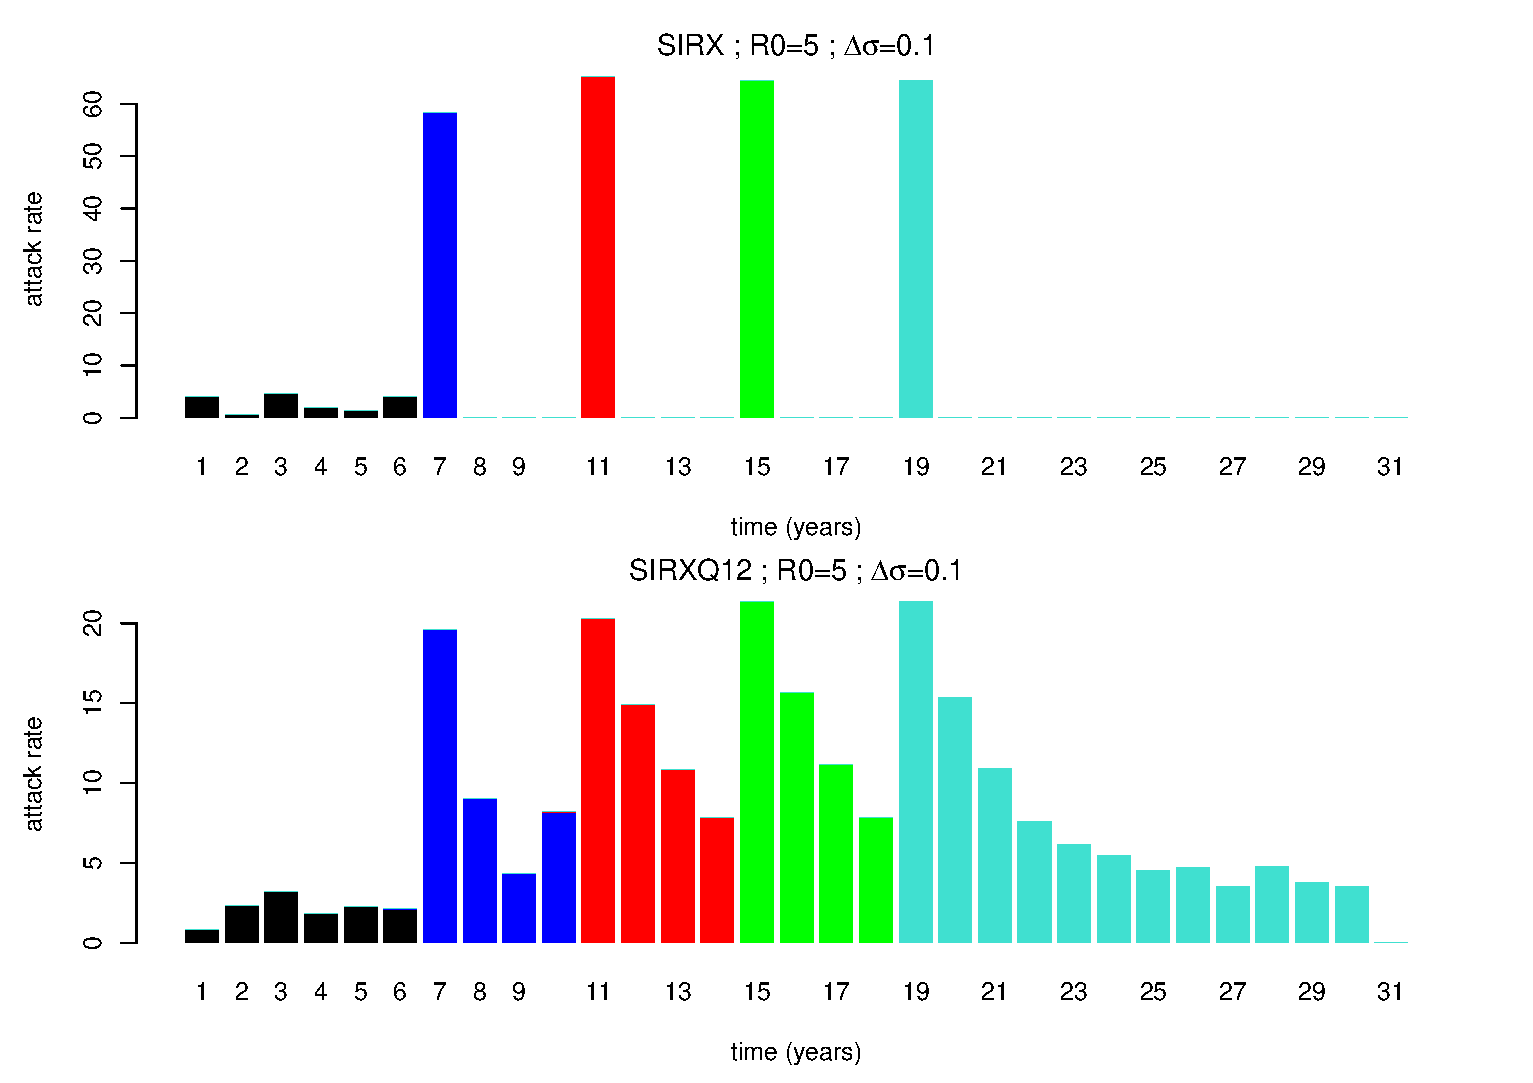
\includegraphics[width=0.9\linewidth]{texte/article3/graph/attack_r05.eps}
  \caption{Evolution of the annual attack rates in Paris for a typical
    realisation of the $SIRX$ (top) and $SIRXQ12$ with immune boosting
    (bottom) stochastic metapopulation models. Parameters are
    identical to figure~\ref{fig:world_sirx} except for $R_0=5$ ;
    $\sigma_X=0.1$ ; $\Delta \sigma=0.1$.}
  \label{fig:attack5}
\end{figure}




% Increasing $R_0$ can improve this situation especially in the $SIRS$
% limit where the effect of cross immune boosting is higher.


\section{Discussion}
\label{sec:discussion}
%a modifier de place


%However, it is difficult to know
%to what extent table \ref{tab:drift_values} estimates are relevant as
%the average antigenic distance between the center of consecutive
%antigenic clusters was used as a measure of a typical antigenic
%distance during antigenic cluster transition for table
%\ref{tab:drift_values} calculation. Given that antigenic cluster are
%relatively ``large'' in antigenic space \citep{Smith2004}, our
%estimates can be overestimated.


%Enfin on sait que: en 29 ans on a mis a jours 19 fois le vaccin (Hay
%2001) soit tous les 1.53 ans (faudrait mettre à jour cette stat)
%Tout d'abord juste pour vérifier:
%si on prend les data de smith on trouve que il faut mettre a jour le
%vaccin en moyenne tous les: 2/1.2=1.67 ans
%avec celle de Russel: tous les 2/2.13=0.94 ans 
%c'est cohérent avec les mise à jour tous les 1.53 ans (heureusement)

%Wild birds and especially aquatic birds of the orders Anseriformes and
%Charadriformes constitute the natural reservoir of influenza A
%viruses. In their reservoir, Influenza A virus possess antigenically
%and genetically diverse hemagglutinin (HA) and neuraminidase (NA)
%subytpes which includes all known influenza A virus HA (16 variants)
%and NA (9 variants). At least 103 of the possible 144 type A influenza
%virus HA-NA combinations have been found in wild birds
%\citep{Dugan2008}
%
%In contrast, influenza B and C virus are mostly present in human. As
%reported by \citet{Webster1992}, modern influenza B and C virus do not
%reassort with influenza A viruses and leave viable progeny. To explain
%this genetic incompatibility, there had to be little or no gene flow
%between human and avian virus gene pools after the introduction of
%avian-derived influenza viruses into human hosts. During a long period
%of isolation, human influenza B and C viruses underwent hosts-specific
%adaptive evolution and accumulated enough mutations that reassortant
%virus were no longer viable.

%This proposal suggests that there have been fundamental changes in the
%ecology of human influenza viruses during human history.  For instance
%\citet{Day2006} report that if evolutionary emergence of past
%pandemics has occurred primarily through viral reassortment in humans,
%then thousands of avian influenza virus infections in humans must have
%occurred each year for the past 250 years.  Due to the decreased
%isolation of human and avian virus gene pools, human influenza viruses
%have been prevented from reaching an evolutionary equilibrium with
%their hosts by an irregular infusion of avian virus genes into the
%human virus gene pool.
%

The current naoH1N1 pandemics illustrates the continuous intrusion of
avian (and swine) influenza genes into the human population. For
instance \citet{Day2006} report that if evolutionary emergence of past
pandemics had primarily occurred through viral reassortment in humans,
then thousands of avian influenza virus infections of humans should
have occurred each year for the past 250 years. In this study, we have
proposed a general framework to handle the dynamics of these
successful perturbations resulting generally in influenza subtype
replacement.
%
At the subtype level, a similar replacement dynamics takes place,
antigenic clusters replacing each other every 1 to 8 years. As
antigenic clusters replacement induce strong selective sweeps
\citep{Koelle2006, Rambaut2008}, this process has recently been
proposed as a key factor to restrict an otherwise ever-growing strain
diversity.

At the heart of our framework is the recognition that influenza
antigenic unit (IAU, either antigenic cluster or subtype) are subject
to gradual antigenic drift \citep{Suzuki2008, Shih2007, Russell2008}.
We coupled an implicit treatment of IAU gradual antigenic drift with
\citet{Koelle2009} proposal of modelling rapidly evolving pathogens by
focusing on the tempo of antigenic change instead of genetic changes.
The resulting model called $SIRX$ allows to track the dynamics of a
considerably lower set of IAU than the previously used multi-strains
models. The few number of IAUs enable us to use the comparatively less
restrictive history-based framework with a sate space scaling
exponentially with the number of IAUs.


%Even if 1977 H1N1 reintroduction resulted in coexistence with H3N2,
%strong interaction between the sutype were reported with H3N2 almost
%completely diseapear in the following year despite H3N2 having undergo
%a major antigenic change event the same year


\subsection{The $SIRX$ framework for drifting co-circulating IAUs}

%Our development of a framework for interacting co-circulating
%antigenic unit subject to within unit antigenic drift adapted to
%influenza has conducted to reject status based model as in their
%simplest form they result in immune boosting dynamics that are
%somewhat incompatible with the original antigenic sin response. Such
%behaviour was reported by \citet{Ballesteros2009} in case of the
%$SBRI$ model without within unit gradual antigenic drift that was used
%by \citet{Gog2002, Koelle2006, Koelle2009, Gog2008}. The $SBRS$ model
%does not present this issue in the absence of gradual antigenic drift
%within antigenic unit however, we have shown that its introduction
%induces cross immune boosting. If cross immune boosting precludes to
%use those status based model in the context of influenza, our analysis
%has revealed interesting invasion threshold properties that highlight
%the importance of transient dynamics and of the time interval of
%antigenic units introduction.

The $SIRX$ model represents an intermediate choice between the $SIRI$
``reinfection'' model of \citet{Goekaydin2007} and the $SIRS$
``gradual loss of immunity'' model of \citep{Pease1987}.

We have shown that this model present an invasion threshold and have
derived a sufficient condition (relevant for a large class of model
allowing a flexible shape of the evolution of the probability of
reinfection due to gradual antigenic drift) that ensures the invasion
of a mutant IAU in a population where a resident IAU is at the endemic
equilibrium. In the absence of functional constraints, this sufficient
condition (SC) states that the invasion threshold occurs only if
infection by a given IAU confers less protection against strains
belonging to the same IAU than against a new IAU. Since this condition
seems like paradoxical we have mostly considered parameter range where
this threshold was absent.

We have then shown that IAU replacement area was maximised for
parameters close to the $SIRI$ limit as $g \to \infty$. Particularly,
absolutely no replacement areas were found for the $SIRS$ limit
($\sigma_X=1$). Further analysis will be necessary to establish to
what extent \citep{Goekaydin2007} reinfection model can constitute a
sufficient representation of an IAU subject to gradual antigenic
drift.

The investigation of the transient dynamics of IAUs replacement using
the $SIRX$ model in a realistic worldwide metapopulation context has
largely confirmed our preliminary determinist analysis.  Successful
IAU replacement are possible only for a small range of parameters. In
particular, our analysis corroborate \citep{Goekaydin2007} results
that within IAU the susceptible reduction factor must be smaller but
close to the reinfection threshold $\sigma_{X}\lesssim 1/R_{0}$. Our
most striking result is the high effect of the mutant IAU immune
escape ($\Delta\sigma$) on the attack rate of the first outbreak as
well as on the post-outbreak refractory period. Successful IAU
replacement followed by realistic recurring epidemics occurred only
for small immune escape values ($\Delta\sigma\thickapprox 5\%$). As we
show below in table~\ref{tab:drift_values} current estimates for
antigenic cluster change are higher, on the order of 15\%. For such
high values, the $SIRX$ model leads to dynamics close to pandemic
situation with unrealistic high attack rates at cluster transitions.

\begin{table}[h!tb]
  \centering
  \begin{tabular}{|c|c|c|}
    \hline
    & \citet{Smith2004} & \citet{Russell2008} \\
    \hline
    \citet{Pease1987} & 8.3 $|$ 18.7 & 4.7 $|$ 10.5 \\
    \hline
    \citet{Finkenstaedt2005} & 12.3 $|$ 27.7 & 6.9 $|$ 15.6 \\
    \hline
  \end{tabular}
  \caption{Percentage of immunity escape corresponding to:
    left value : 2 antigenic units change (equivalent to a fourfold difference in
    hemagglutination inhibition (HI) assay titer which is considered
    as a sufficient antigenic difference to warrant a vaccine update)
    right value : the average antigenic distance between the center of
    consecutive clusters (4.5$\pm$1.3 in \citet{Smith2004}).
    Calculation were performed by  using \citet{Smith2004}
    and \citet{Russell2008} estimates of the rate of evolution of
    antigenic drift at the phenotypic level (using hemagglutination
    inhibition (HI) assay titer) (resp. 1.2  and 2.13 unit per year) as well as \citet{Pease1987} and
    \citet{Finkenstaedt2005} inference of the rate of loss of immunity
    following an influenza infection (resp. 5\% and 7.4\% per year).}
  \label{tab:drift_values}
\end{table}


Various factors can mitigate this high sensitivity to $\Delta\sigma$
and we have shown that a functional trade-off between transmission
rate and immune escape ability could greatly help to reduce this gap.
However, this trade-off hypothesis is more difficult to model and will
necessitate additional processes to account for compensatory
mutations. In this context the model of \citet{Gog2008} is a
significant improvement but should be re-analysed without the
limitation induced by the $SBRI$ framework.

We have also shown that the addition of a temporary period of full
protection with immune boosting, as suggested by \citet{Ferguson2003},
could improve the situation mostly by reducing the sharpness of the
epidemics and transforming area where both the invading and the
resident IAUs go extinct into successful replacement area.
%
%Interestingly this effect is particularly present in the $SIRS$ limit
%($\sigma_X=1$) for within IAU antigenic drift rates close to values
%inferred from experiments \citep{Pease1987} or data
%\citep{Finkenstaedt2005} ($1/g \approx 10-25$ years$^{-1}$) and
%$R_0\approx 5$, both parameters values where the effect of immune
%boosting are particularly present. Strikingly for this parameter area,
%and due to the existence of the invasion threshold of eq.
%\eqref{eq:threshold} $\Delta\sigma$ of the order of values reported in
%table~\ref{tab:drift_values} leads to successful IAU replacements.
%
From a more biological standpoint we have shown that there were three
ways to introduce this temporary period. Referring to section
\ref{sec:Q} we think that assumption $Q_{1}$ is biologically
reasonable and empirically supported since it occurs after infection
and that cellular immunity targeted toward conserved proteins is well
known to participate viral clearance \citep{Grebe2008}.
%
By contrast, assumption $Q_{2}$ is less evident as it is unknown to
what extent exposure that do not lead to infection can trigger a
cellular immune response. For the same reason, we doubt on the
relevance of assumption $Q_{3}$ as it concern host with an effective
immunity where efficient long lived antibodies can repress the virus
before viral replication ensure sufficient stimulation to trigger a
cellular immune response. 
%
Recent studies tacking influenza A replacement patterns have
emphasized the need for such temporary full-protective period
(\citet{Ferguson2003,Minayev2008,Minayev2009,Tria2005}) without
precisely explaining the underlying biological assumptions. Our study
reveals a significant effect of assumption $Q_{2}$, and calls for
better clarifications before using $Q_{2}$ and especially $Q_{3}$.



%For instance, \citet{Minayev2008,Minayev2009} refer to
%\citet{Ferguson2003} while introducing a short-lived
%strain-transcending immunity. Looking more precisely to their
%equations reveals that they use the assumption $Q_{1}$, a variant of
%the assumption $Q_{2}$ (due to the way the host's immune repertoire is
%updated following exposure) and the more problematic assumption
%$Q_{3}$. Moreover, it seems like there is an inconsistency in their
%equations when introducing this temporary strain-transcending
%immunity. Equation $(4.2)$ of \cite{Minayev2009} (\textit{resp.}
%equation $(2.6)$ of \cite{Minayev2009a}) implies that infection can
%come from a strain already in the immune repertoire: in that case host
%does not become infectious yet develops 6 months strain-transcending
%immunity ($Q_{3}$). But the authors also precise that equation $(2.1)$
%in both papers remains unchanged which is inconsistent with equation
%$(4.2)$ (\textit{resp.} $(2.6)$) since equation $(2.1)$ implies that
%hosts can not be infected or develop 6 months strain-transcending
%immunity if they are challenged by strains already in their immune
%repertoire. In other words, equation $(2.1)$ does not support the
%assumption $Q_{3}$ whereas equations $(4.2)$ (\textit{resp.} $(2.6)$)
%does. The direct consequence of this is an overestimation of the force
%of infection for co-circulating strains. Since this temporary
%full-protection plays a crucial role in their model it must be tested
%if this inconsistency modify the epidemiological and evolutionary
%dynamics and by how much. Note also that this inconsistency can only
%be removed by modifying equation $(2.1)$, thus fully supporting
%assumption $Q_{3}$.

Recent analysis (\citet{Kryazhimskiy2007,Ballesteros2009}) have
revealed a similar issue with the multi-strains status-based model
with reduced infectivity ($SBRI$) as introduced by \citet{Gog2002,
  Koelle2006}. \citet{Ballesteros2009} have for instance showed that
the $SBRI$ model results in significant cross immune boosting in
contradiction with the original antigenic sin \citep{Kim2009}. The
$Q_2$ and $Q_3$ mechanism discussed previously are somewhat comparable
to the cross immune boosting induces by the $SBRI$ with the important
difference that boosting is only temporary (but strain transcending)
and not mediated by a lifelong acquisition of effective immunity to
antigenically distant strain in better agreement with the original
antigenic sin.

In summary, our analysis reveals that the core of the replacement
dynamics of drifting IAU (and therefore of selective sweep as the main
mechanism of strain diversity reduction \citep{Koelle2006}) is already
present in the simple $SIRX$ model but that this model lacks a
mechanism to reduce the sharpness of the epidemics following IAUs
transitions. Such mechanisms could refer to functional constraints or
short-lived strain-transcending immunity with immune boosting although
this latter assumption call for more empirical evidence.


We also suggest that introducing an additional source of heterogeneity
in our model would greatly improve its ability to reproduce IAU
replacement as observed in data. It will be necessary for instance to
relax the assumption of global mixing at the patch (city) level.
Before such an analysis we think that our results cannot be used to
infer level of heterotypic partial cross-immunity as the previously
highlighted strong sensitivity to immune escape can induce important
overestimation of this parameter of tremendous importance for public
health and pandemic preparedness. By focusing on the phenotype level,
the $SIRX$ framework presented here and its mathematical structure is
particularly adapted to be used with recently developed ``plug and
play'' inference technique \citep{Ionides2006, Toni2009}. Such an
analysis will be valuable to disentangle between the various process
previously described. Particularly, we wonder to what extent complex
immune boosting mechanisms ($SBRI$ model or $Q123$) are still
necessary in a more heterogeneous local spatial context.


\subsection{Noisy gradual antigenic drift or punctuated immune escape}

As a last point, in its current form the presented models given their
high sensitivity to immune escape of the mutant tends to support noisy
gradual antigenic drift instead of strong punctuated immune escape. It
is striking to observe how the $SIRX$ model or especially the $SIRXQ_{12}$
model with immune boosting perturbed with small immune escape (of
the order of 5\%) produced by IAU transitions are able to
successfully reproduce observed influenza time series both
qualitatively and quantitatively. \citet{Finkenstaedt2005} analysis of
French ILI data tends also to support this conclusion of noisy gradual
antigenic drift as their inferred immune escape parameters are far
lower than values expected during antigenic cluster transitions even
with the presence of a scaling exponent to handle deviation from
homogeneous mixing. Given the recent discussion on the fact that
influenza antigenic evolution is punctuated or gradual (\textit{e.g}
\citep{Wolf2006, Shih2007, Suzuki2008}) and the recent discovery that
purely gradual antigenic drift is sufficient to induce strong epidemic
variability due to non linear dynamics effects (Ballesteros et al 2009
, submitted), the use of the statistical framework described
above will be of tremendous interest to gain definitive insights with
a mechanistic basis on these long standing questions.

%sinon discutter des parametres
%bcp de cross immuntiy pour les pandemies ???
%biais de loi d'action de masse ?

%%

\section*{Acknowledgements}
This work was partially funded by the R\'egion Ile-de-France and the
“ANR-Agence Nationale de la Recherche – The French National Research
Agency” under the project ANR 05SEST01802 BIOSCOPE.



%%% Local Variables: 
%%% mode: latex
%%% TeX-master: "../../phD"
%%% End: 
